\documentclass[11 pt]{article} 
\usepackage[left=2cm, top=2cm, right=2cm, bottom=2.5cm, footskip=.5cm]{geometry}
\usepackage{graphicx}
\usepackage{subcaption} 
\usepackage{subfig}
\usepackage{amsmath}
\usepackage{url}
\usepackage{booktabs}
\usepackage{units}
\usepackage{enumitem}
\usepackage{listings}
\usepackage{float}
\usepackage{booktabs}
%\usepackage{hyperref}
\usepackage[svgnames]{xcolor}
\definecolor{mygray}{rgb}{0.9,0.9,0.9}

\lstset{language=R,
	basicstyle=\small\ttfamily,
	stringstyle=\color{DarkGreen},
	otherkeywords={0,1,2,3,4,5,6,7,8,9},
	morekeywords={TRUE,FALSE},
	deletekeywords={data,frame,length,as,character},
	keywordstyle=\color{blue},
	commentstyle=\color{DarkGreen},
	frame=single,
	backgroundcolor=\color{mygray},
	numbers=left, 
}

\author{Natalia Zuniga-Garcia}
\title{Exercises 5 Sparsity}
\date{October 15, 2017}

\begin{document}

\maketitle


Broadly speaking, there are three ways to think about enforcing sparsity in a statistical model.\footnote{In this context, sparsity means that some of the parameters are zero.  This is different from the notion of sparsity considered previously, where some of the \textit{features} in a regression problem were zero.}
\begin{itemize}
	\item The old-school frequentist way, based on classical hypothesis tests (chi-squared tests, $F$ tests, likelihood ratio tests, etc), perhaps coupled with greedy algorithms for model selection.
	\item The Bayesian way, in which sparsity is baked into the prior distribution on some parameter \footnote{E.g. http://www-stat.wharton.upenn.edu/~edgeorge/Research\_papers/fastN96.pdf}
	\item The new-school frequentist way, based on penalizing the likelihood function in a way that encourages sparsity, and computing a \textit{maximum penalized likelihood} estimate.
\end{itemize}

These viewpoints all have their advantages and disadvantages.  One the major advantages of the penalized-likelihood view of sparsity (especially versus the Bayesian view) is scalability to large data sets.  That makes it particularly suited to big-data applications, which is why we'll pursue it here, and for much of the rest of the course.

\section{Penalized likelihood and soft thresholding}

\begin{enumerate}[label=(\Alph*)]
\item Define the function
\begin{equation}
\label{eqn:soft_thresholding}
S_\lambda(y) = \arg \min_{\theta} \; \frac{1}{2}(y - \theta)^2 + \lambda | \theta | \, .
\end{equation}
The intuition here is that $\theta$ is a parameter of a statistical model, and $y$ is data.   The first (quadratic) term rewards good fit to the data, while the second term rewards $\theta$ for being ``simpler'' (i.e.~closer to zero).  $S_\lambda(y)$ returns an estimate for $\theta$ that blends these two goals.

First show (in a trivial one- or two-liner) that the quadratic term in the objective above is the negative log likelihood of a Gaussian distribution with mean $\theta$ and variance 1.  

\vspace{2mm}
\textbf{Solution}

The Gaussian PDF is:

$$ f(y,\mu, \sigma) = \frac{1}{\sqrt{2 \pi \sigma^2}} \exp ^ {\frac{(y - \mu)^2}{2 \sigma^2}}$$

A Gaussian distribution with mean $\theta$ and variance 1 is:
$$ f(y,\theta, 1) = \frac{1}{\sqrt{2 \pi}} \exp ^ {\frac{(y - \theta)^2}{2}}$$

The likelihood for a single y is: 
$$ L(\theta| y,1) =   \frac{1}{\sqrt{2 \pi}} \exp ^ {\frac{(y - \theta)^2}{2}}$$

And the negative log-likelihood is: 
$$ l(\theta| y,1) =  - \bigg(-\frac{1}{2}log(2 \pi) - \frac{1}{2}(y - \theta)^2 \bigg) = C + \frac{1}{2}(y - \theta)^2$$

Where, $C= \frac{1}{2}log(2 \pi)$ is a constant. We can observe that the negative log-likelihood contains the quadratic form in Equation (1).  

\vspace{10mm}

Then prove that 
$$
S_\lambda(y) = \mbox{sign}(y) \cdot (|y| - \lambda)_+ \, ,
$$
where $a_+ = \max(a,0)$ is the positive part of $a$.  This is a basic exercise in sub-differential calculus
\footnote{http://ocw.mit.edu/courses/electrical-engineering-and-computer-science/6-253-convex-analysis-and-optimization-spring-2012/lecture-notes/MIT6\_253S12\_lec12.pdf},
 if you happen to know this subject.  But I am not assuming that you do, and you can also prove the statement using ordinary differential calculus if you split it up into cases ($\theta>0$, $\theta<0$, and $\theta=0$).\footnote{If you know about constrained optimization, you could also introduce a slack variable $z$ and write the objective as
	$$
	\frac{1}{2}(y - \theta)^2 + \lambda | z | \, ,
	$$
	and then do the minimization subject to the constraint that $\theta = z$.}  

\vspace{2mm}
\textbf{Solution}

First, we try to minimize the objective function by calculation its derivative with respect to $\theta$ and equalizing it to zero as follow,

$$ \frac{\partial}{\partial \theta}S_\lambda(y) = 0 \Rightarrow  \frac{\partial }{\partial \theta} \bigg(\frac{1}{2}(y - \theta)^2 + \lambda | \theta |\bigg) =-(y - \theta) + \lambda sign (\theta) = 0 $$
$$ \Rightarrow  \theta = y - \lambda sign (\theta) $$

Now, we split this into three cases:

\begin{itemize}
	\item Case 1. $\theta>0$, $\theta = y - \lambda \Rightarrow$ 
	Then we have that $y > \lambda$
	\item Case 2. $\theta<0$, $\theta = y + \lambda \Rightarrow$ 
	Then we have that $y < - \lambda$
	\item Case 3. $\theta=0$, $ y = \lambda \Rightarrow$ 
	Then we have that $|y| < \lambda$
\end{itemize}

Which can be written as:
$$ S_\lambda(y) = \mbox{sign}(y) \cdot (|y| - \lambda)_+ \, $$

\newpage

To build intuition, you should try plotting the objective in Equation \ref{eqn:soft_thresholding} for various $y$ and $\lambda$, and verifying that $S_\lambda(y)$ indeed obtains the minimum.\footnote{Recall the ``curve'' function in R, which acts like a graphing calculator.}

\vspace{2mm}
\textbf{Solution}

The solution is presented in the file $Part\_1A.R$,

\lstinputlisting[language = R, firstline=4, lastline=21]{R_Code/Part_1A.R}

\begin{figure}[H]
	\begin{center}
		\begin{subfigure}[h]{0.3\linewidth}
			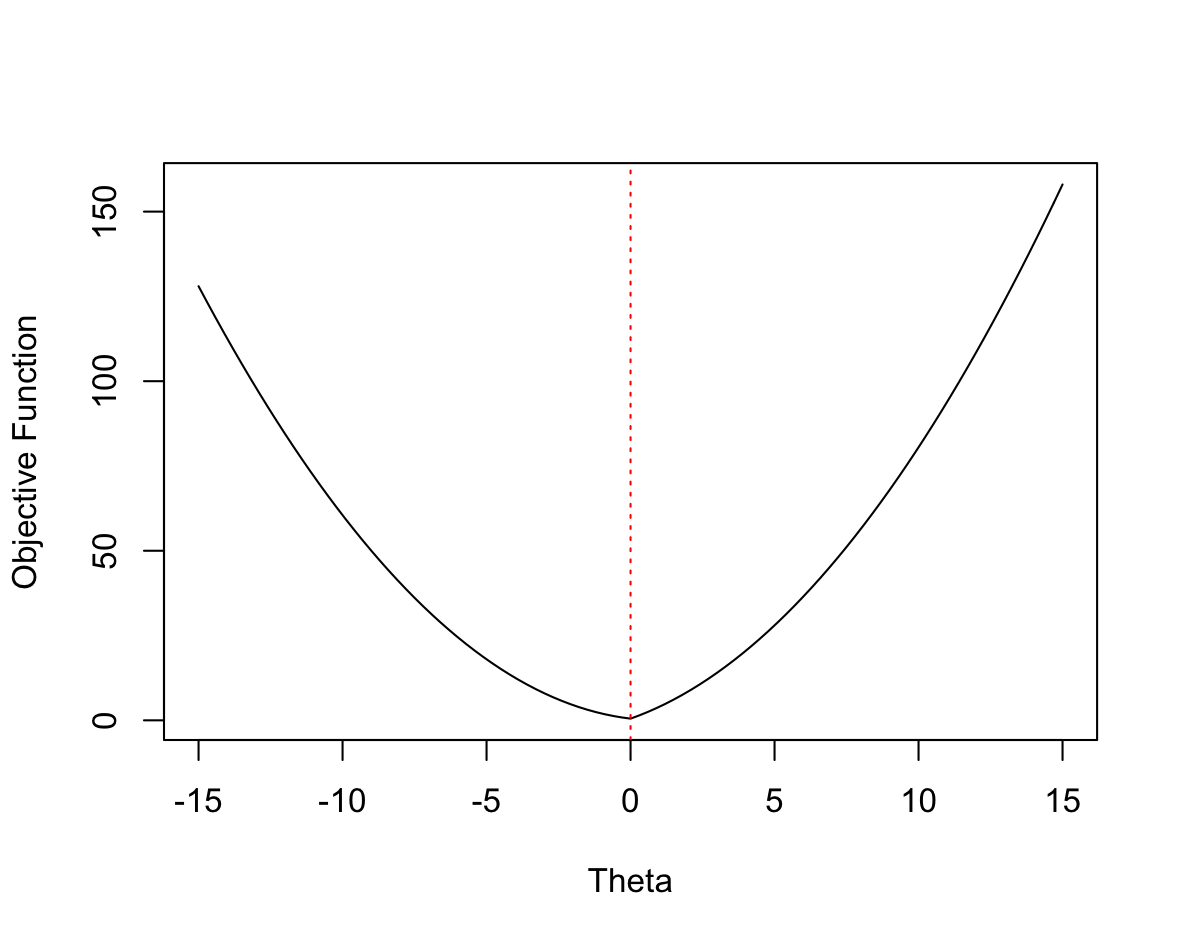
\includegraphics[width=\linewidth]{R_Code/Fig/P1A-12.png}
			\caption{$y=-1$ and $\lambda=2$}
		\end{subfigure}
		\begin{subfigure}[h]{0.3\linewidth}
			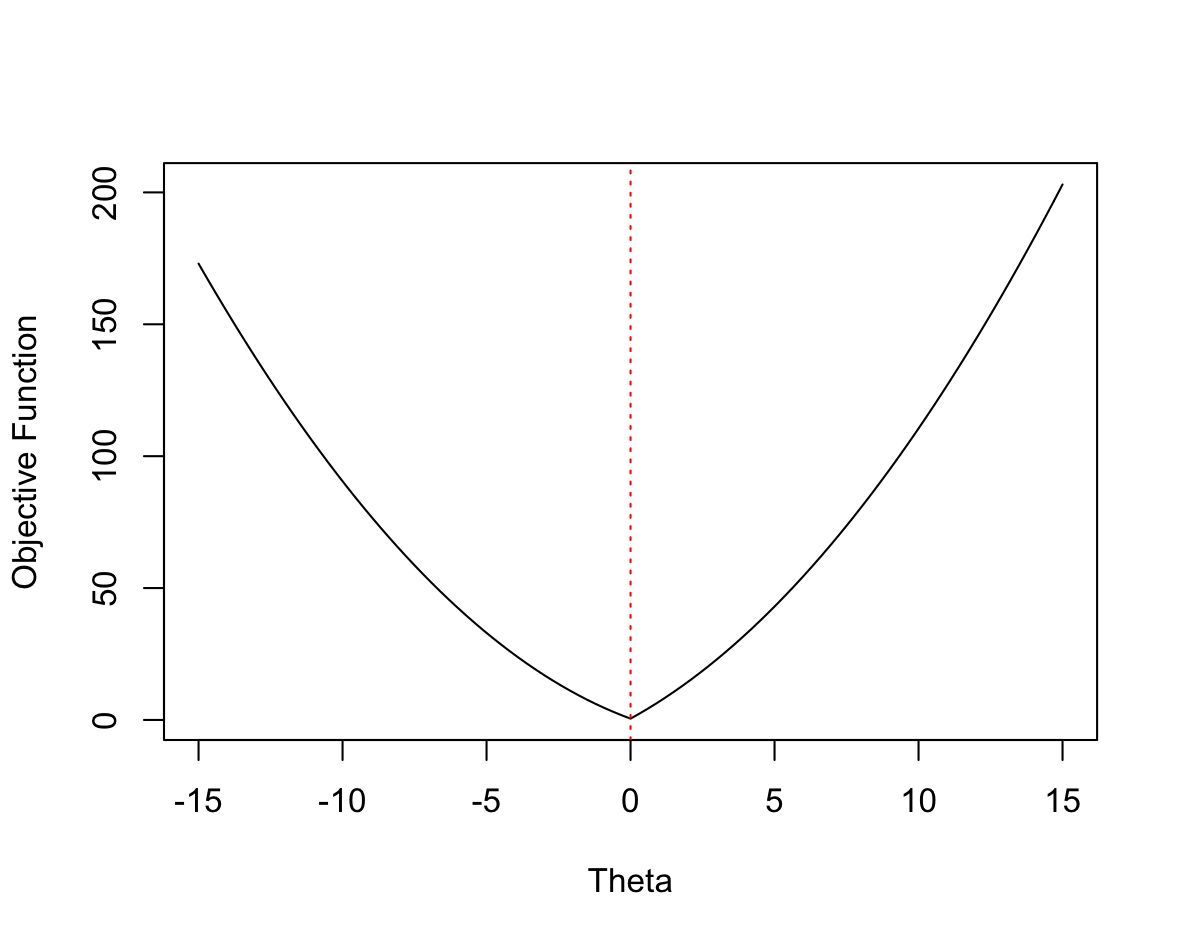
\includegraphics[width=\linewidth]{R_Code/Fig/P1A-15.png}
			\caption{$y=-1$ and $\lambda=5$}
		\end{subfigure}
		\begin{subfigure}[h]{0.3\linewidth}
			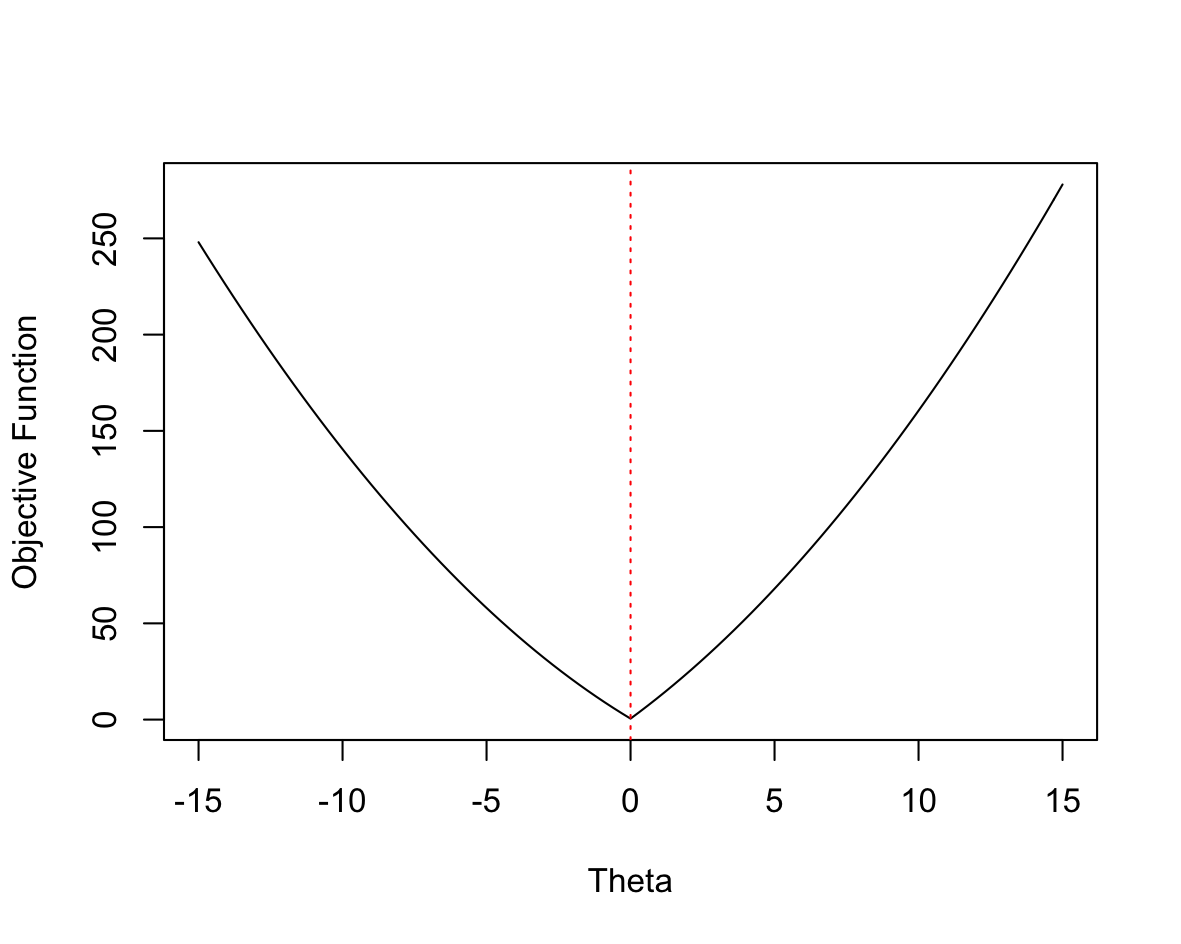
\includegraphics[width=\linewidth]{R_Code/Fig/P1A-110.png}
			\caption{$y=-1$ and $\lambda=10$}
		\end{subfigure}
		\begin{subfigure}[h]{0.3\linewidth}
			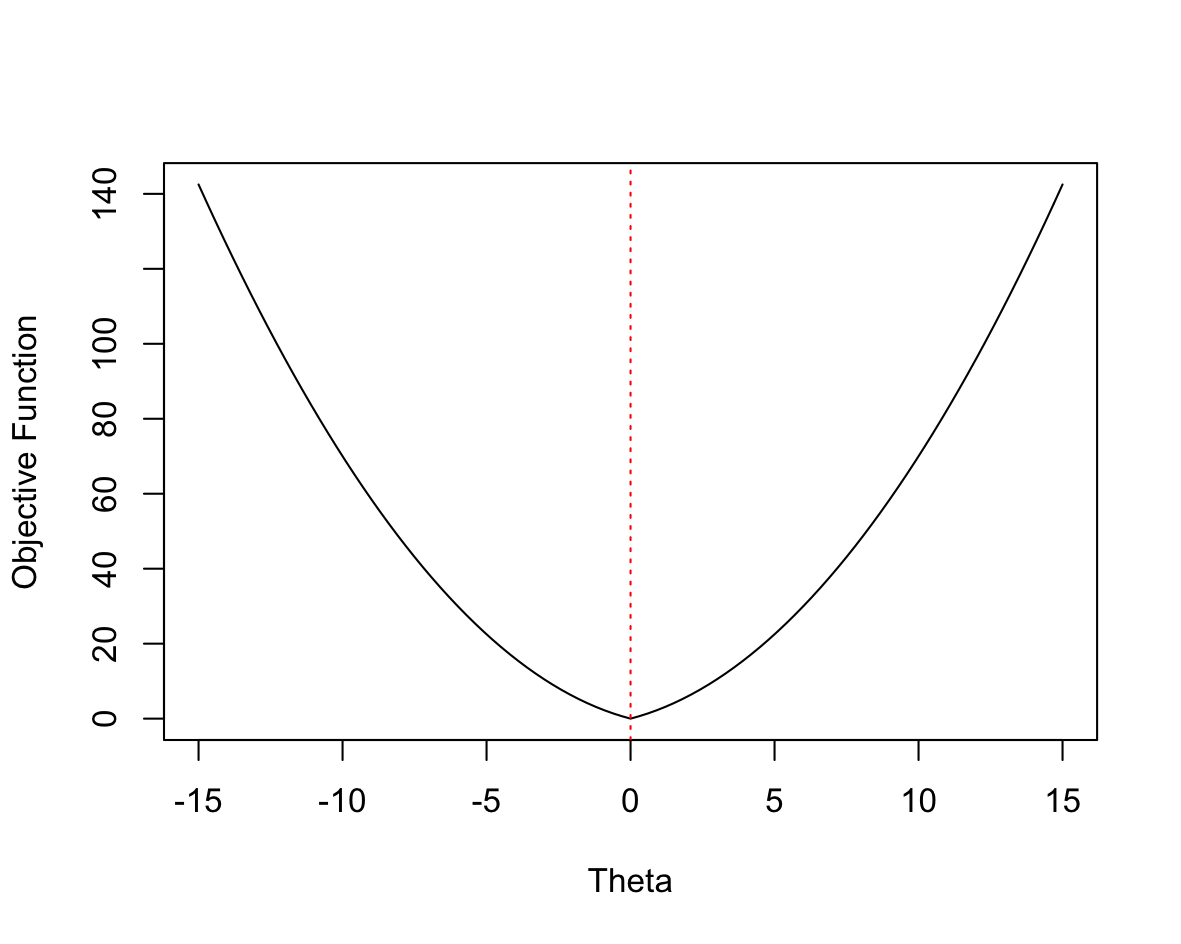
\includegraphics[width=\linewidth]{R_Code/Fig/P1A02.png}
			\caption{$y=0$ and $\lambda=2$}
		\end{subfigure}
		\begin{subfigure}[h]{0.3\linewidth}
			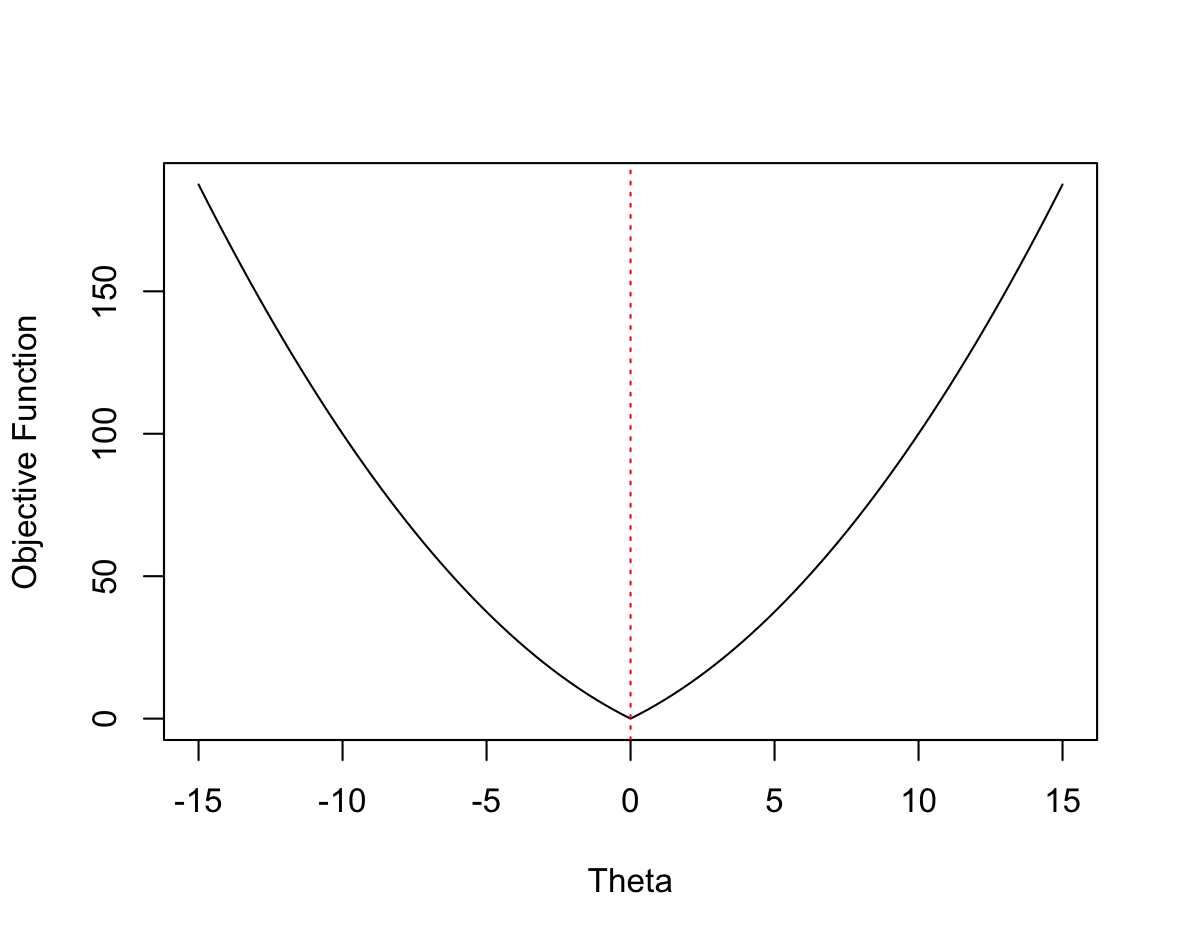
\includegraphics[width=\linewidth]{R_Code/Fig/P1A05.png}
			\caption{$y=0$ and $\lambda=5$}
		\end{subfigure}
		\begin{subfigure}[h]{0.3\linewidth}
			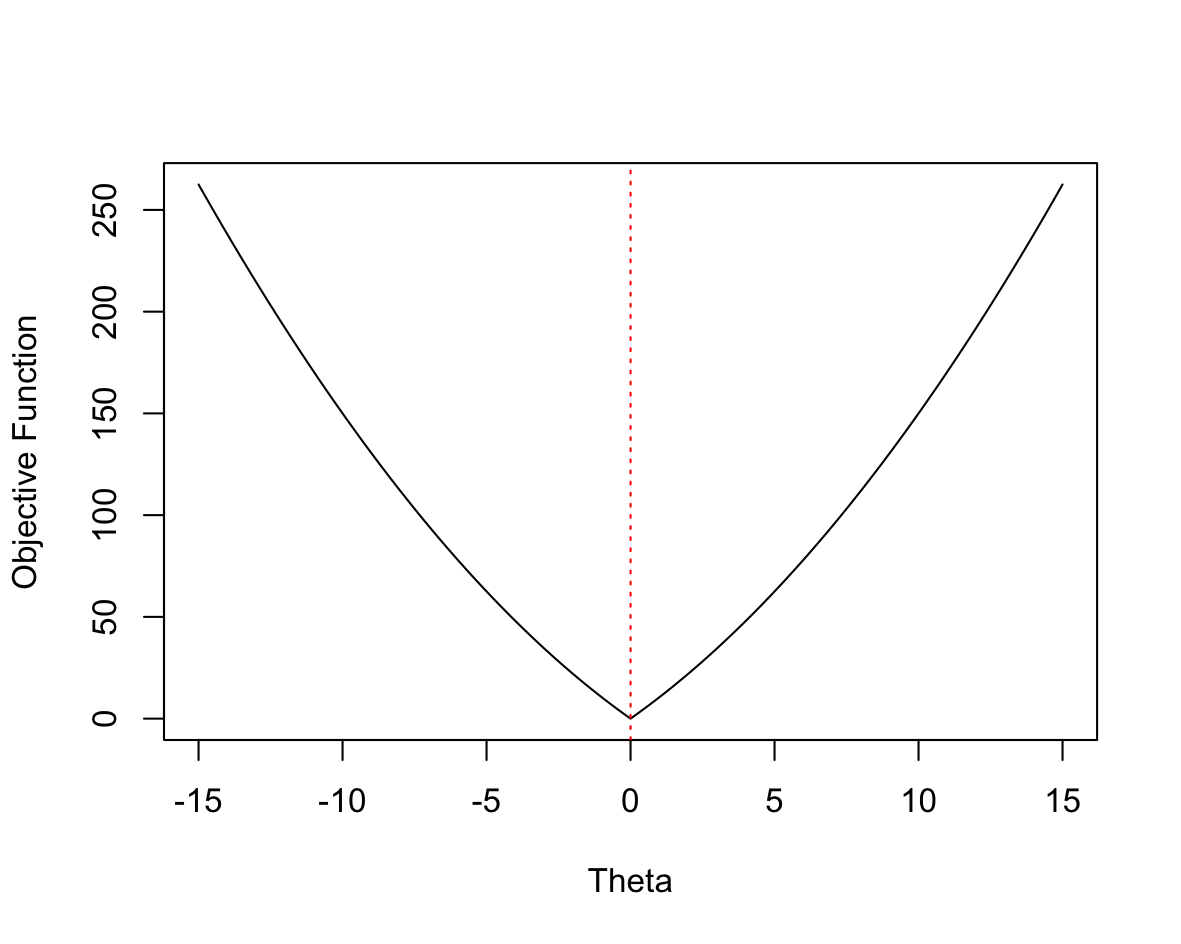
\includegraphics[width=\linewidth]{R_Code/Fig/P1A010.png}
			\caption{$y=0$ and $\lambda=10$}
		\end{subfigure}
		\begin{subfigure}[h]{0.3\linewidth}
			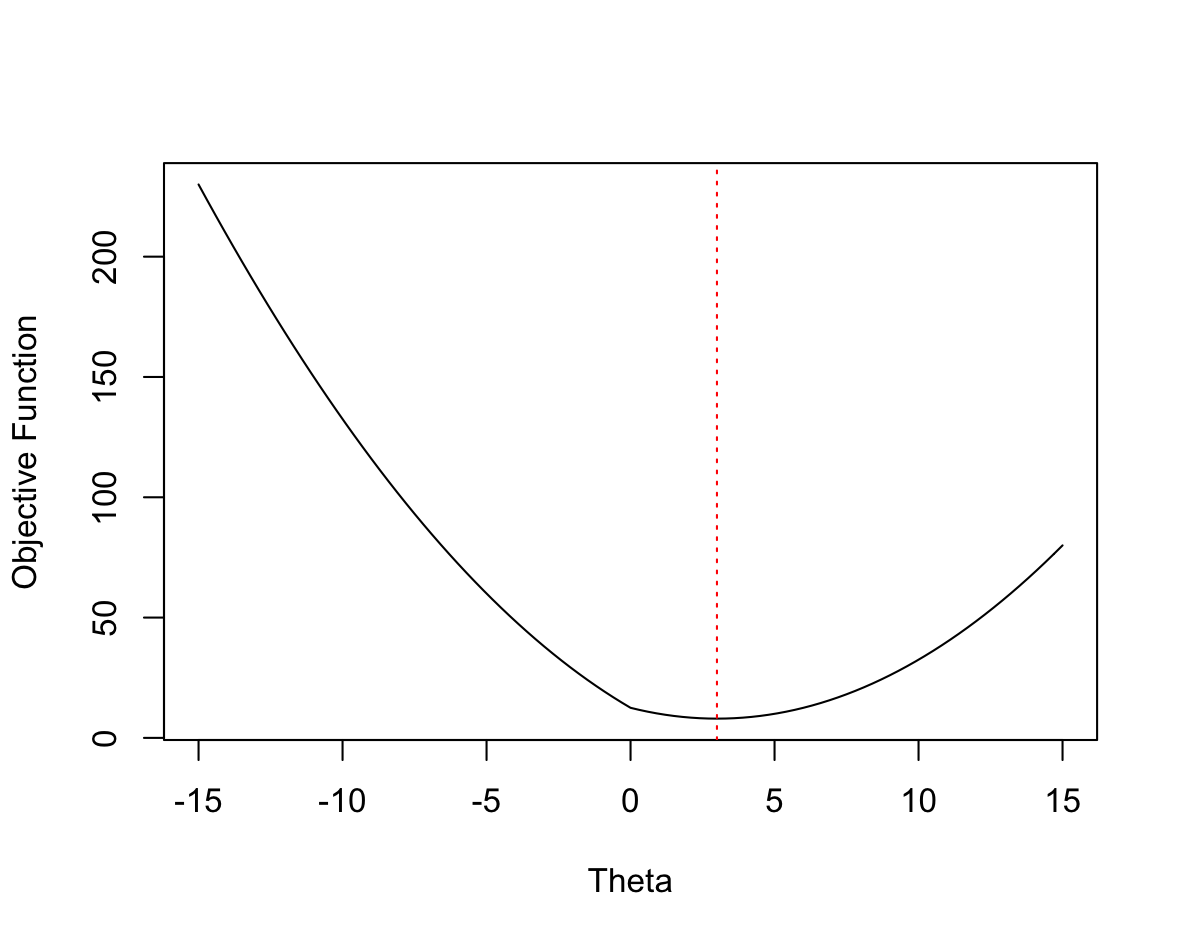
\includegraphics[width=\linewidth]{R_Code/Fig/P1A52.png}
			\caption{$y=5$ and $\lambda=2$}
		\end{subfigure}
		\begin{subfigure}[h]{0.3\linewidth}
			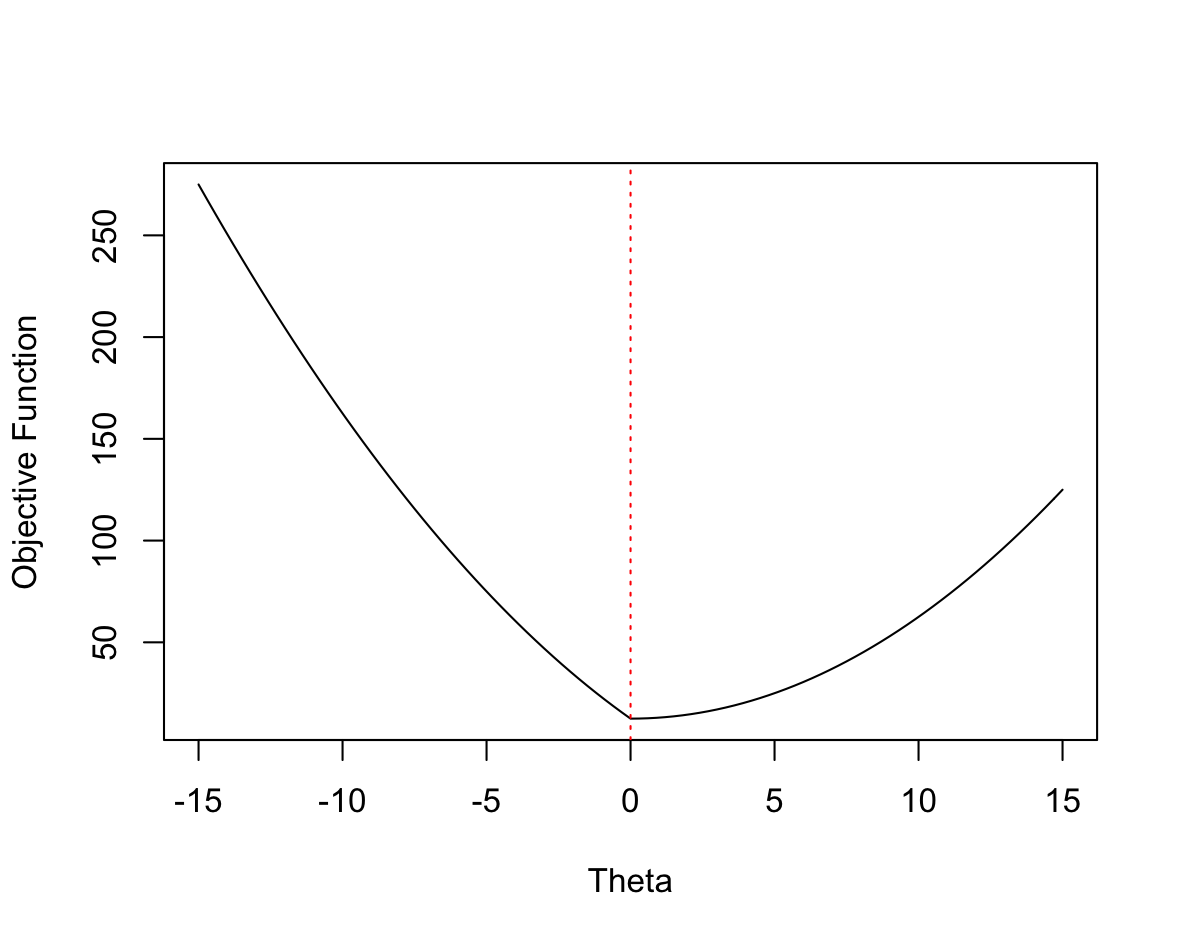
\includegraphics[width=\linewidth]{R_Code/Fig/P1A55.png}
			\caption{$y=5$ and $\lambda=5$}
		\end{subfigure}
		\begin{subfigure}[h]{0.3\linewidth}
			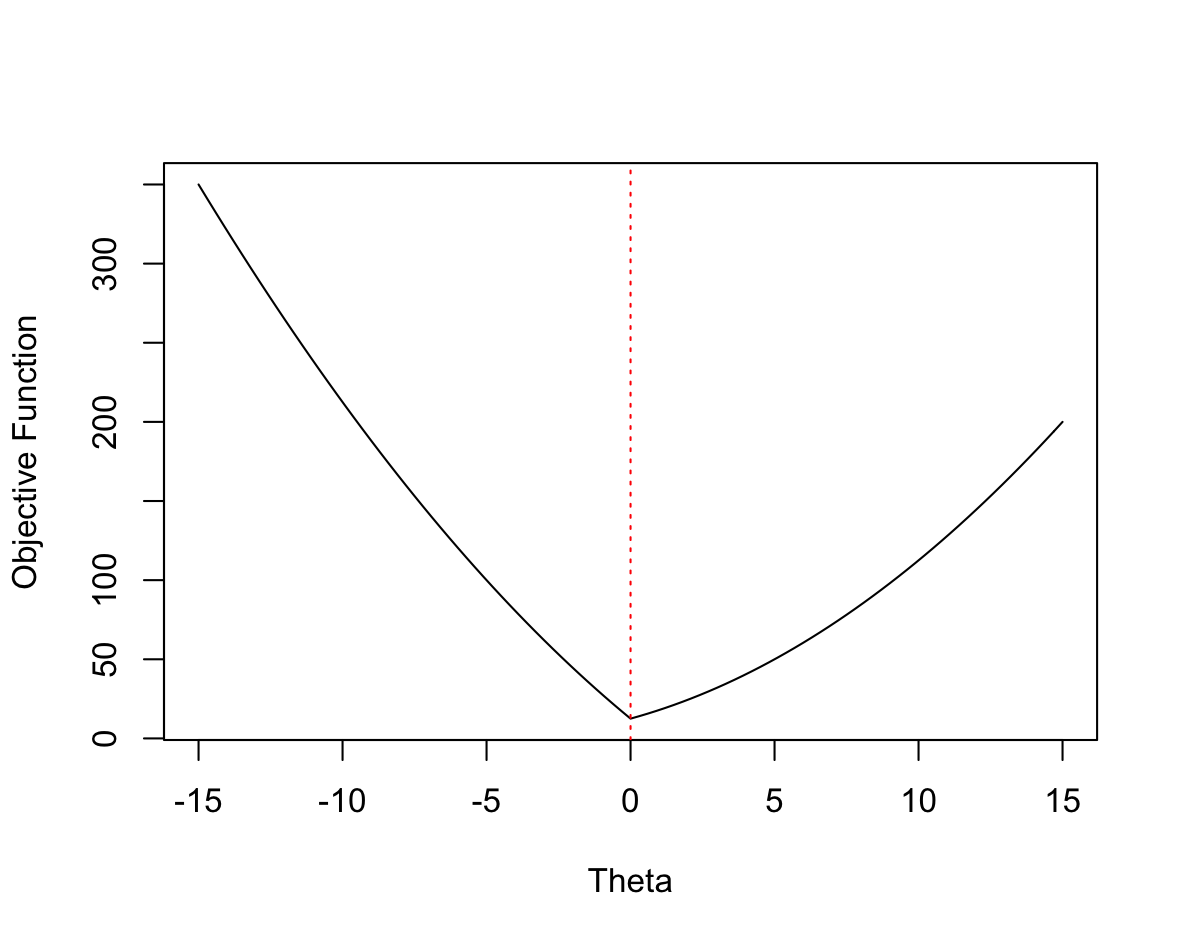
\includegraphics[width=\linewidth]{R_Code/Fig/P1A510.png}
			\caption{$y=5$ and $\lambda=10$}
		\end{subfigure}
		\caption{Objective Function and $S_\lambda(y)$ with different values of $y$ and $\lambda$}
		\label{fig:Fig1}
	\end{center}
\end{figure}


\newpage

$S_\lambda(y)$ is called the \textit{soft thresholding} function with parameter $\lambda$.  Plot this as function of $y$ for a few different parameters of $\lambda$.  You'll see how it encourages sparsity in a ``soft'' way, especially if you compare it to the hard-thresholding function
$$
H_{\lambda}(y) = 
\left \{
\begin{array}{ll}
y & \mbox{if $y \geq \lambda$} \\
0 & \mbox{otherwise} \, .
\end{array}
\right.
$$

\vspace{2mm}
\textbf{Solution}

The solution is presented in the file $Part\_1A.R$,

\lstinputlisting[language = R, firstline=23, lastline=43]{R_Code/Part_1A.R}

\begin{figure}[H]
	\begin{center}
		\begin{subfigure}[h]{0.4\linewidth}
			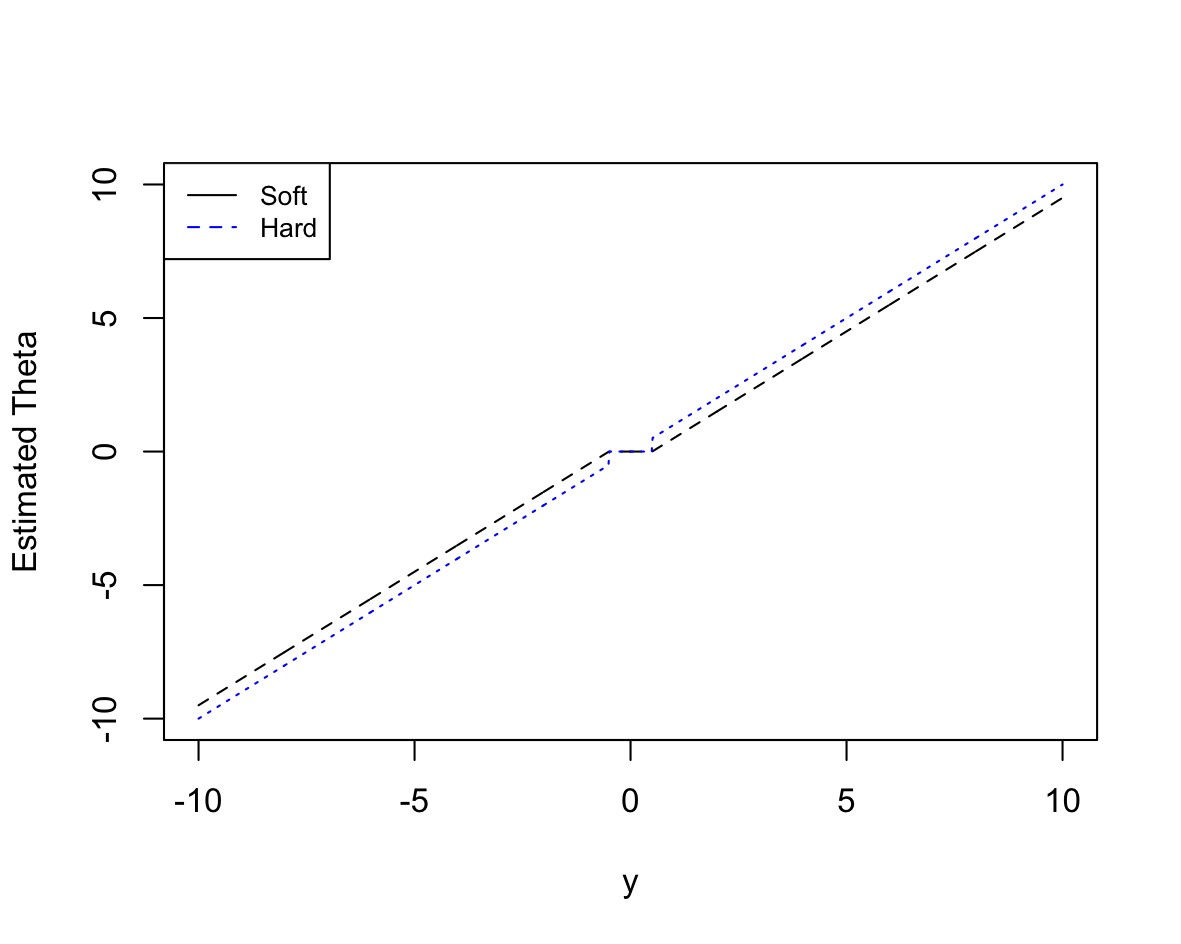
\includegraphics[width=\linewidth]{R_Code/Fig/P1AA05.png}
			\caption{$\lambda=0.5$}
		\end{subfigure}
		\begin{subfigure}[h]{0.4\linewidth}
			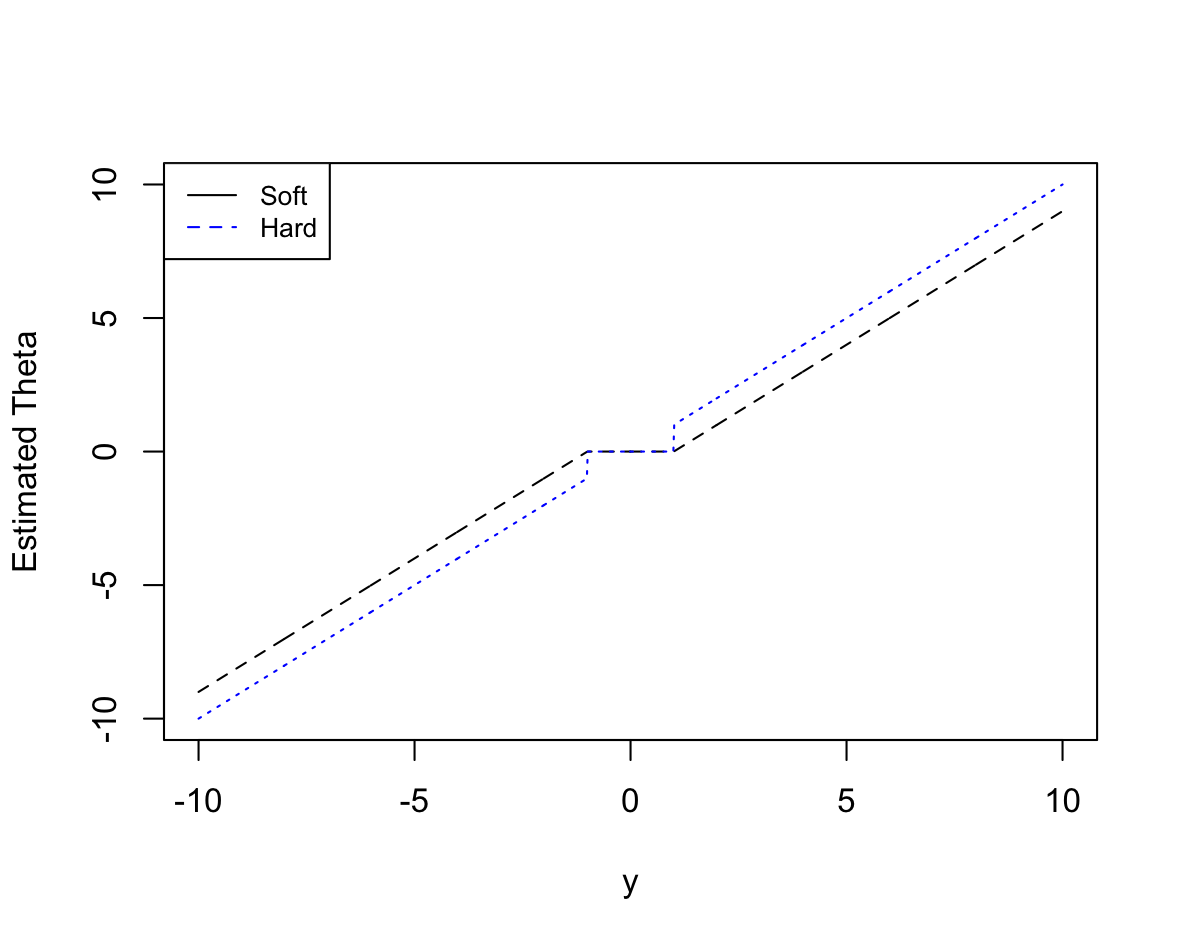
\includegraphics[width=\linewidth]{R_Code/Fig/P1AA1.png}
			\caption{$\lambda=1$}
		\end{subfigure}
		\begin{subfigure}[h]{0.4\linewidth}
			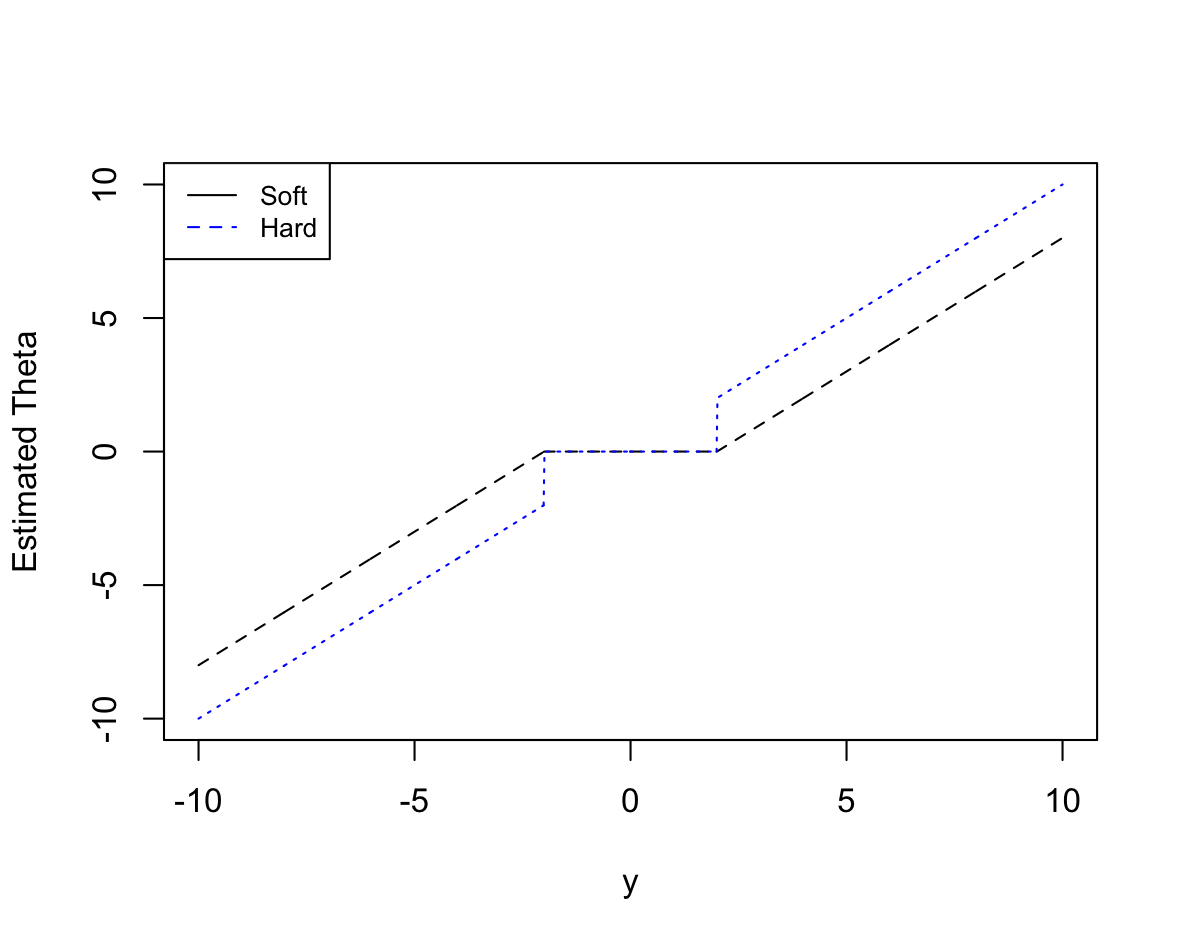
\includegraphics[width=\linewidth]{R_Code/Fig/P1AA2.png}
			\caption{$\lambda=2$}
		\end{subfigure}
		\begin{subfigure}[h]{0.4\linewidth}
			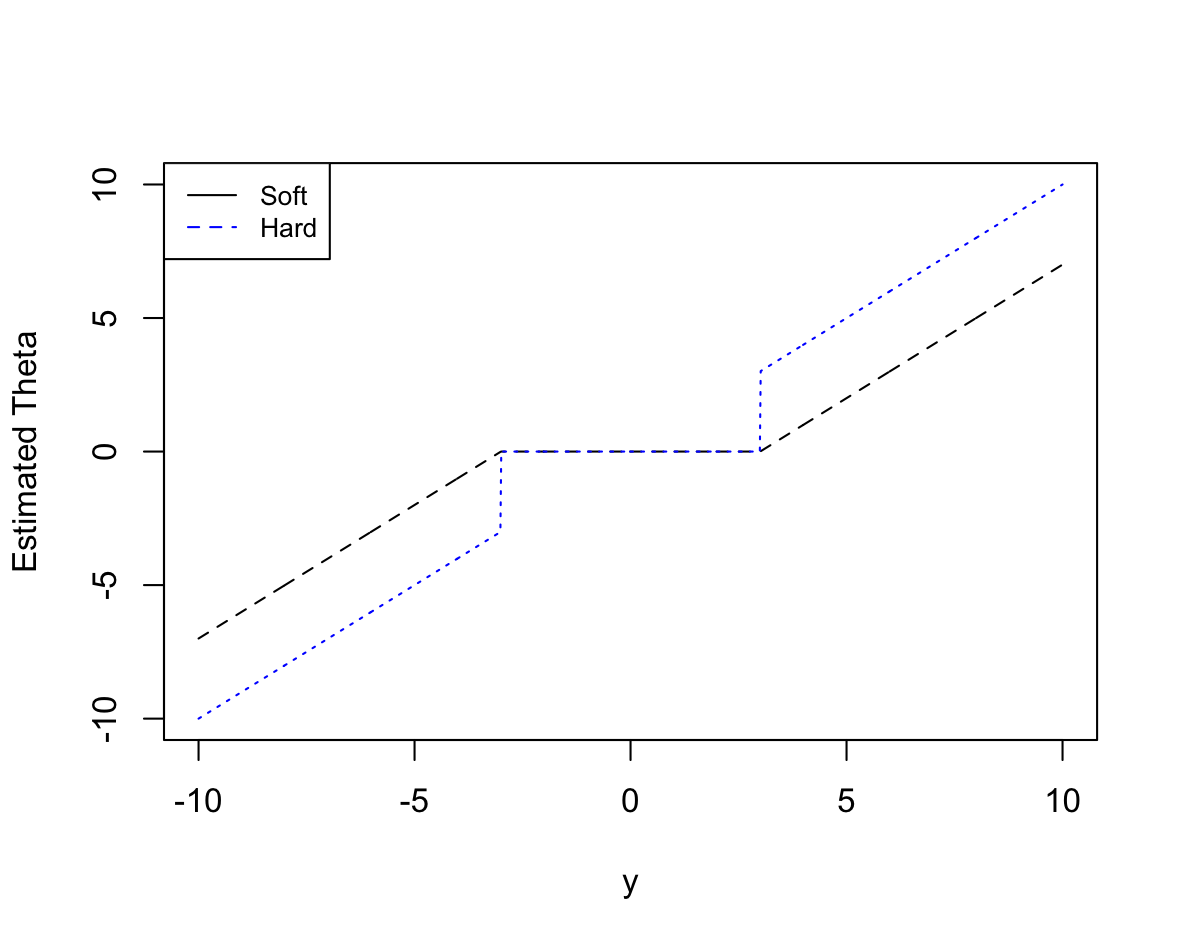
\includegraphics[width=\linewidth]{R_Code/Fig/P1AA3.png}
			\caption{$\lambda=3$}
		\end{subfigure}
		\begin{subfigure}[h]{0.4\linewidth}
			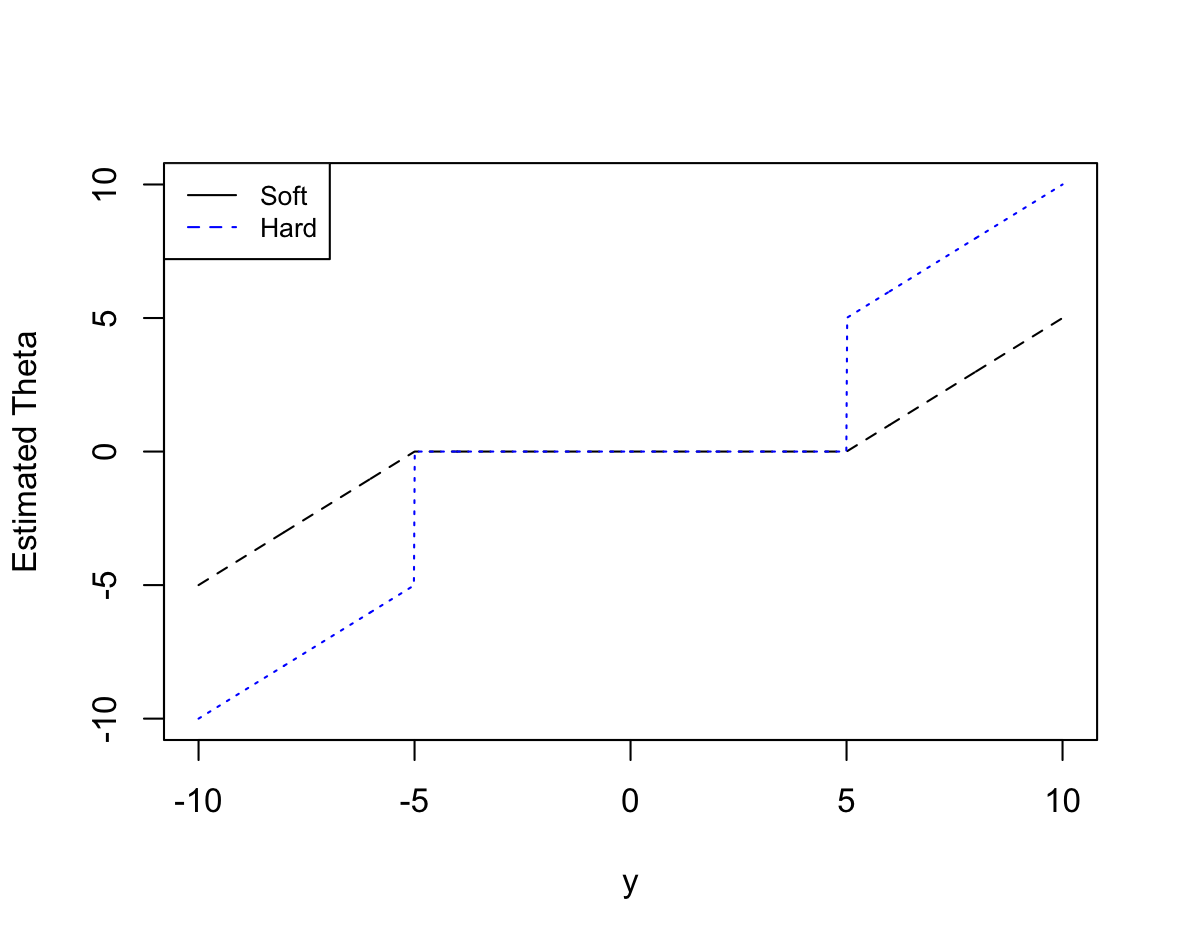
\includegraphics[width=\linewidth]{R_Code/Fig/P1AA5.png}
			\caption{$\lambda=5$}
		\end{subfigure}
		\begin{subfigure}[h]{0.4\linewidth}
			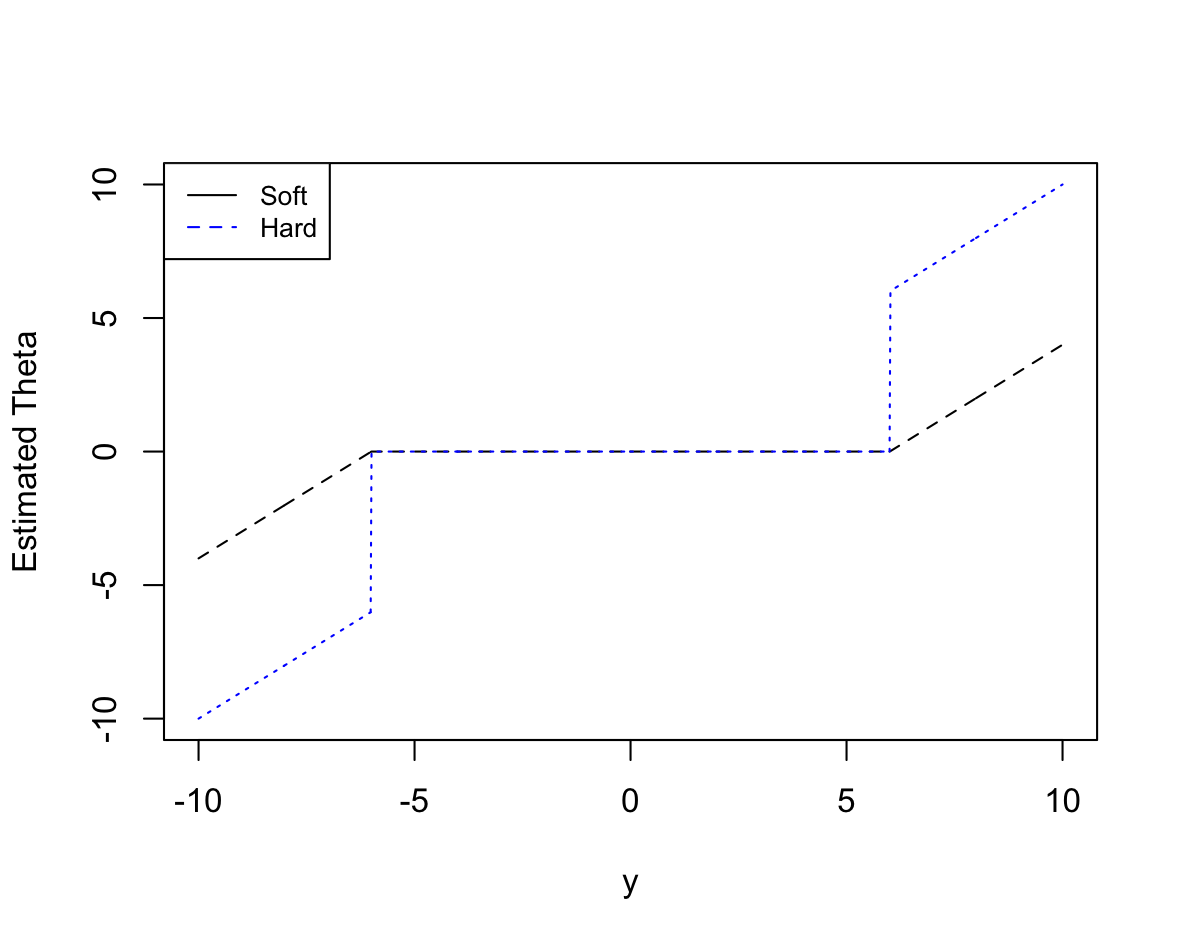
\includegraphics[width=\linewidth]{R_Code/Fig/P1AA6.png}
			\caption{$\lambda=6$}
		\end{subfigure}
		\caption{Soft-thresholding and hard-thresholding functions with different  $\lambda$ values}
		\label{fig:Fig1}
	\end{center}
\end{figure}



\newpage
\item Here's a simple toy example to illustrate how soft thresholding can be used to enforce sparsity in statistical models.

Suppose we observe data from the following statistical model:
$$
(z_{i} \mid \theta_i) \sim N(\theta_i, \sigma^2_i) \, .
$$
That is, there are $n$ different means $\theta_i$, and we observe 1 normally distributed observation for each one.  We allow that each observation has a different variance $\sigma^2_i$; for now we'll assume these are known.  This is called the Gaussian sequence model, or the normal-means problem.  It looks like a toy problem, but is surprisingly useful \footnote{\url{http://statweb.stanford.edu/~imj/GE06-11-13.pdf}} in a wide variety of applications, from curve fitting to image denoising to genome-wise association studies.\footnote{The simplest example is probably curve-fitting using an orthogonal basis of functions, like Fourier polynomials or wavelets; see the link provided.}

Now suppose we believe that a lot of the $\theta_i$'s are zero---i.e.~that the vector $\theta = (\theta_1, \ldots, \theta_n)^T$ is sparse.  Consider an estimator for each $\theta_i$ of the form
$$
\widehat{\theta}(y_i) = S_{\lambda \sigma_i^2}(y_i) \, ,
$$
where $S$ is the soft thresholding operator defined above with parameter $\lambda \sigma_i$.  (Side question: why $\lambda \sigma_i^2$ for the soft-thresholding parameter?)

\textbf{Solution}

Because for the objective function we are scaling by the standard deviation:

$$\frac{1}{2}\bigg(\frac{y - \theta}{\sigma}\bigg)^2 + \lambda | \theta | \Rightarrow \frac{1}{2}(y - \theta)^2 + \lambda \sigma_i^2 | \theta | $$

\vspace{10mm}
Try the following intuition-building exercise.
\begin{enumerate}[label=\arabic*.]
	\item Choose some sparse vector $\theta$ and the corresponding $\sigma_i^2$'s (it's OK for them all to be equal).  You have freedom in deciding what the nonzero elements of $\theta$ should be, and how sparse it should be.  (Ideally there would be some tunable parameter that you could use to ratchet up or down the sparsity level.)\\
	\textbf{Solution}\\
	The solution is presented in the file $Part\_1B.R$,
	\lstinputlisting[language = R, firstline=6, lastline=18]{R_Code/Part_1B.R}
	\item Simulate one data point $(z_i \mid \theta_i) \sim N(\theta_i, \sigma^2_i)$ for each $\theta_i$.
	\lstinputlisting[language = R, firstline=20, lastline=29]{R_Code/Part_1B.R}
	\item Compute $\widehat{\theta}(y_i) = S_{\lambda \sigma_i^2}(y_i)$ across a discrete grid of different $\lambda$ values.  Plot $\widehat{\theta}(y_i)$ versus $\theta_i$, and observe how the soft-thresholding function both \emph{selects} certain $\theta_i$'s by sparsifying the estimate, as well as \emph{shrinks} the nonzero estimates $\widehat{\theta}(y_i)$ towards 0 (and towards each other).
	\lstinputlisting[language = R, firstline=31, lastline=58]{R_Code/Part_1B.R}
	\begin{figure}[H]
		\begin{center}
			\begin{subfigure}[h]{0.3\linewidth}
				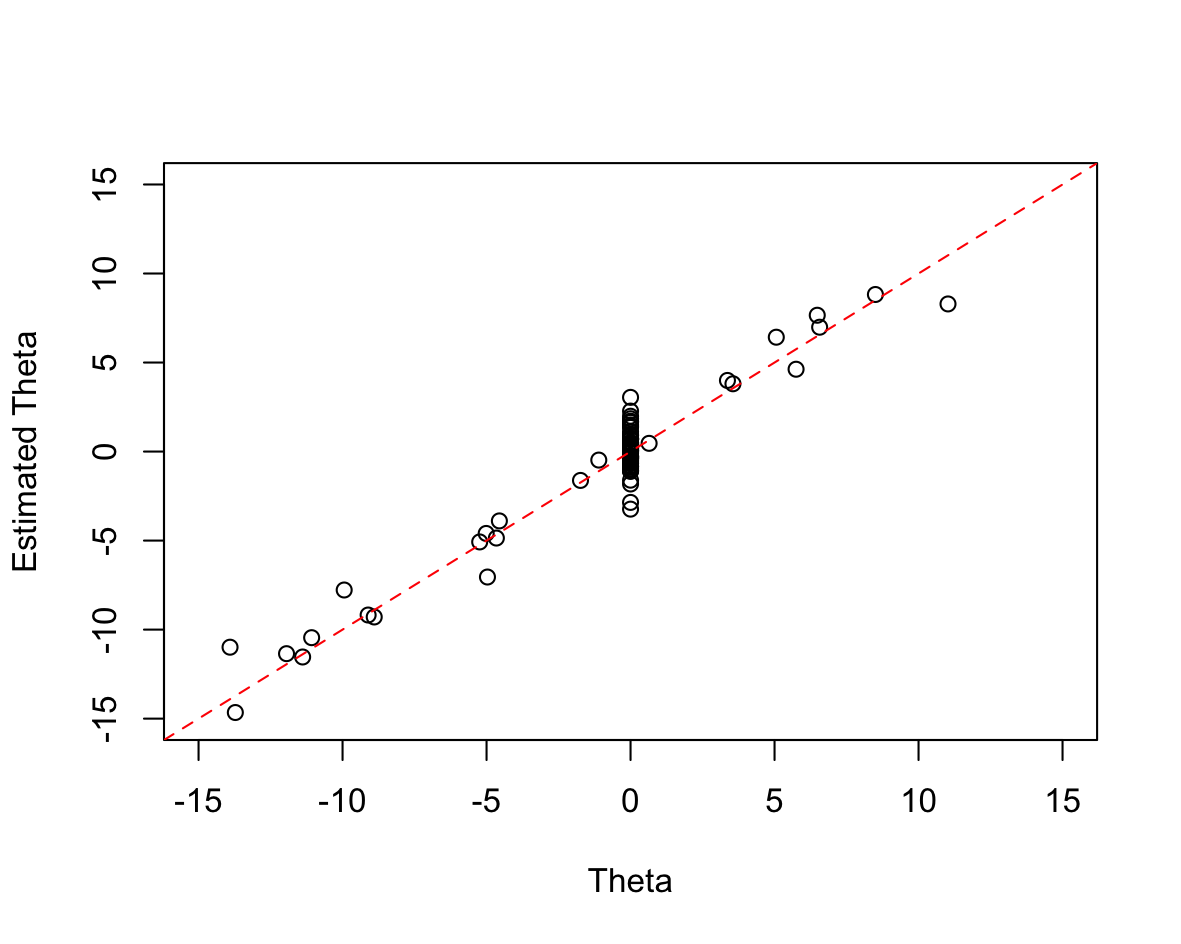
\includegraphics[width=\linewidth]{R_Code/Fig/P1B_K_03_l_0.png}
				\caption{$\lambda=0$ and $K=0.3$}
			\end{subfigure}
			\begin{subfigure}[h]{0.3\linewidth}
				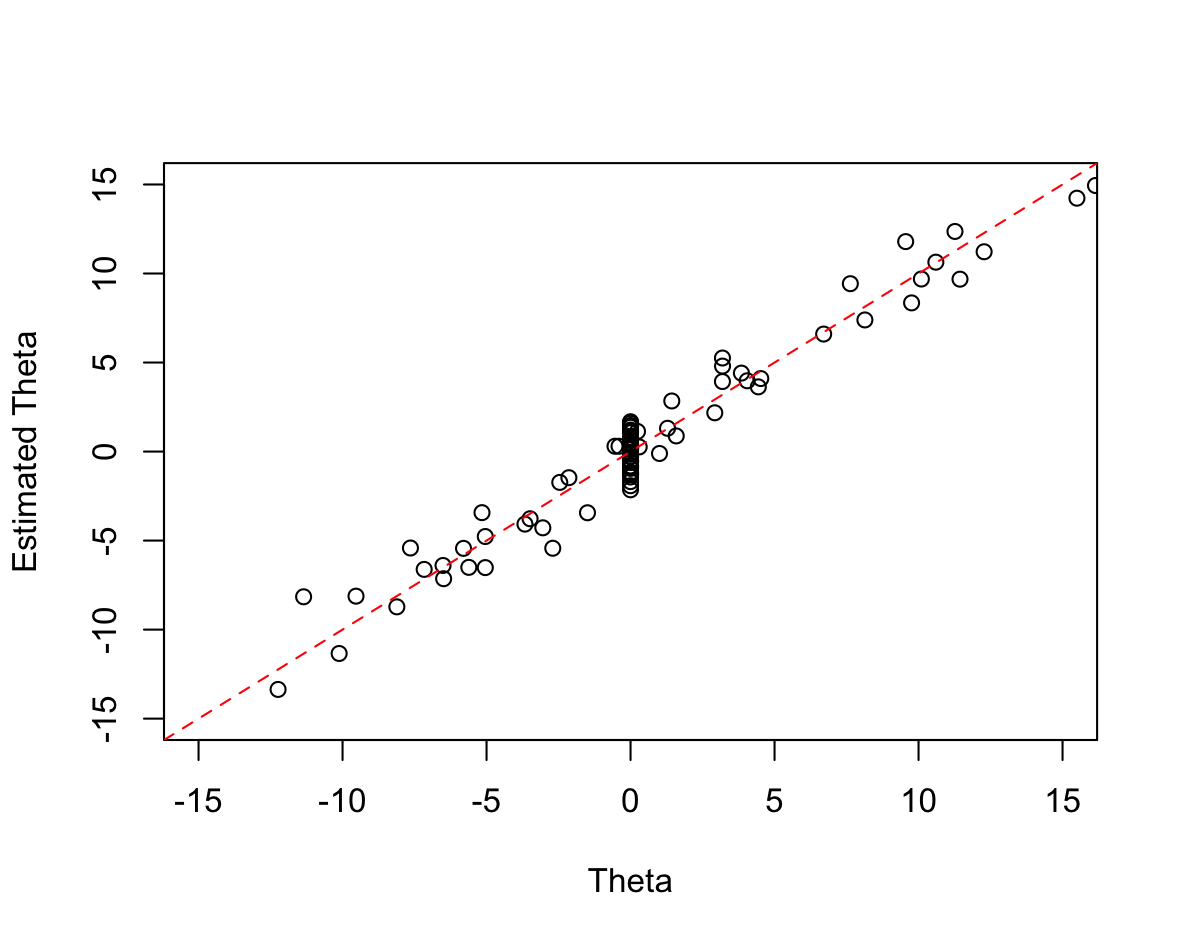
\includegraphics[width=\linewidth]{R_Code/Fig/P1B_K_05_l_0.png}
				\caption{$\lambda=0$ and $K=0.5$}
			\end{subfigure}
			\begin{subfigure}[h]{0.3\linewidth}
				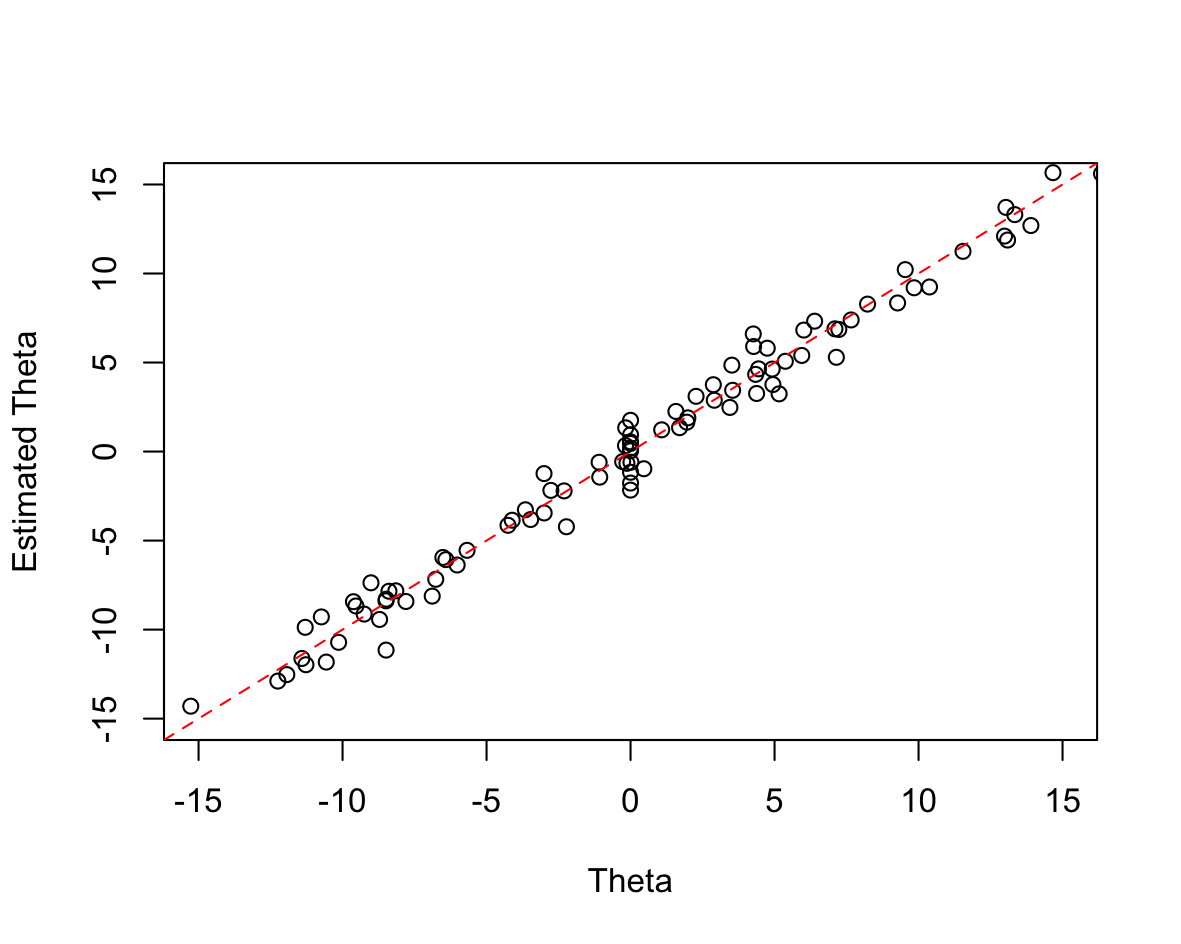
\includegraphics[width=\linewidth]{R_Code/Fig/P1B_K_09_l_0.png}
				\caption{$\lambda=0$ and $K=0.9$}
			\end{subfigure}
			\begin{subfigure}[h]{0.3\linewidth}
				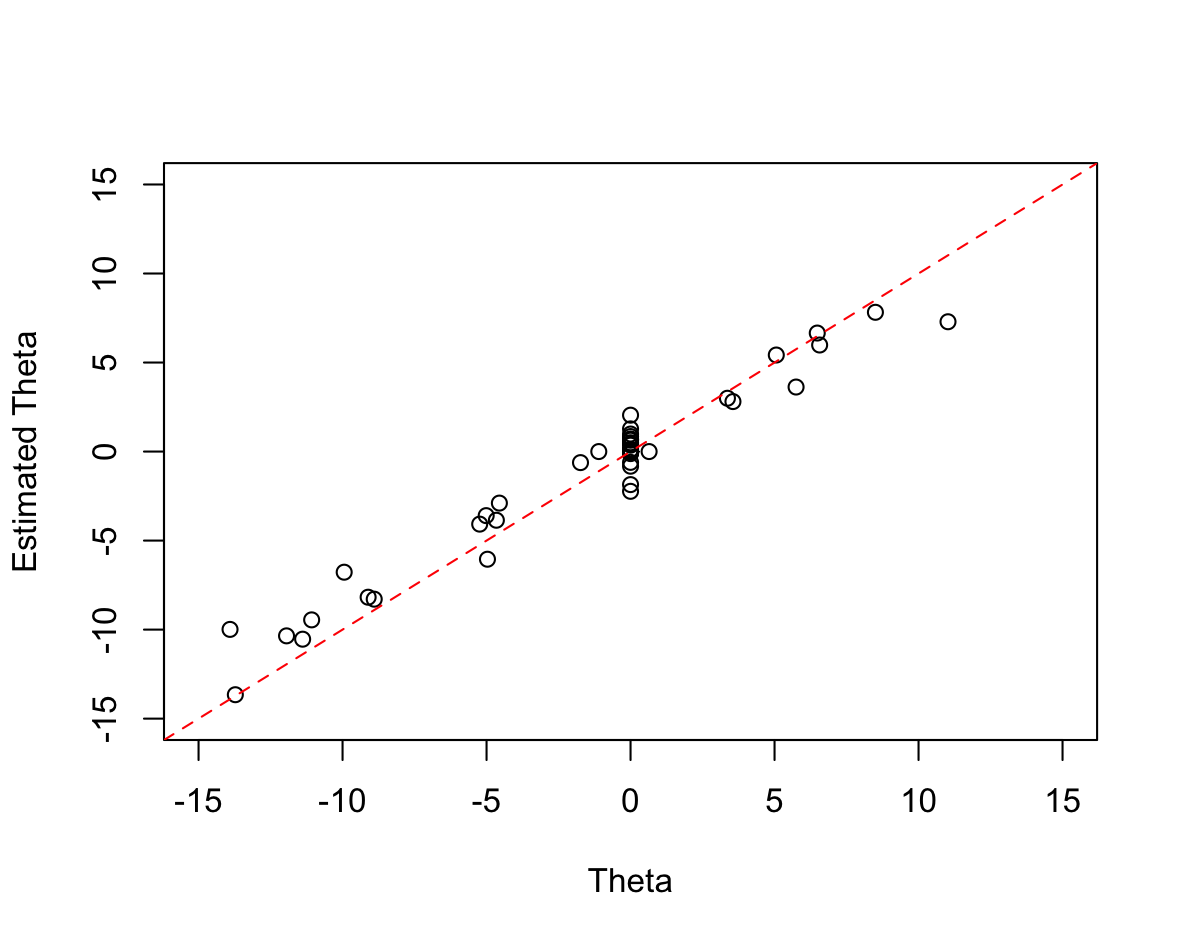
\includegraphics[width=\linewidth]{R_Code/Fig/P1B_K_03_l_1.png}
				\caption{$\lambda=1$ and $K=0.3$}
			\end{subfigure}
			\begin{subfigure}[h]{0.3\linewidth}
				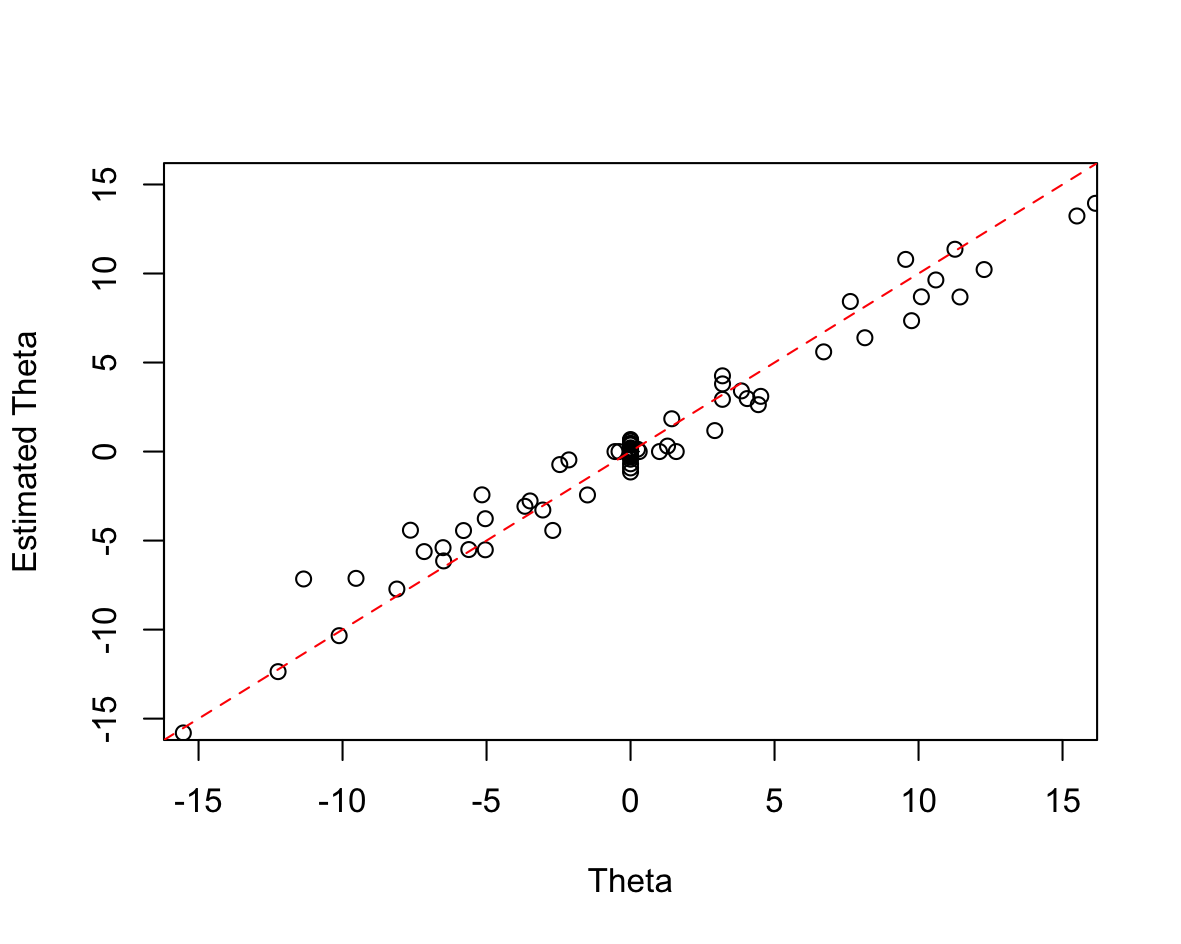
\includegraphics[width=\linewidth]{R_Code/Fig/P1B_K_05_l_1.png}
				\caption{$\lambda=1$ and $K=0.5$}
			\end{subfigure}
			\begin{subfigure}[h]{0.3\linewidth}
				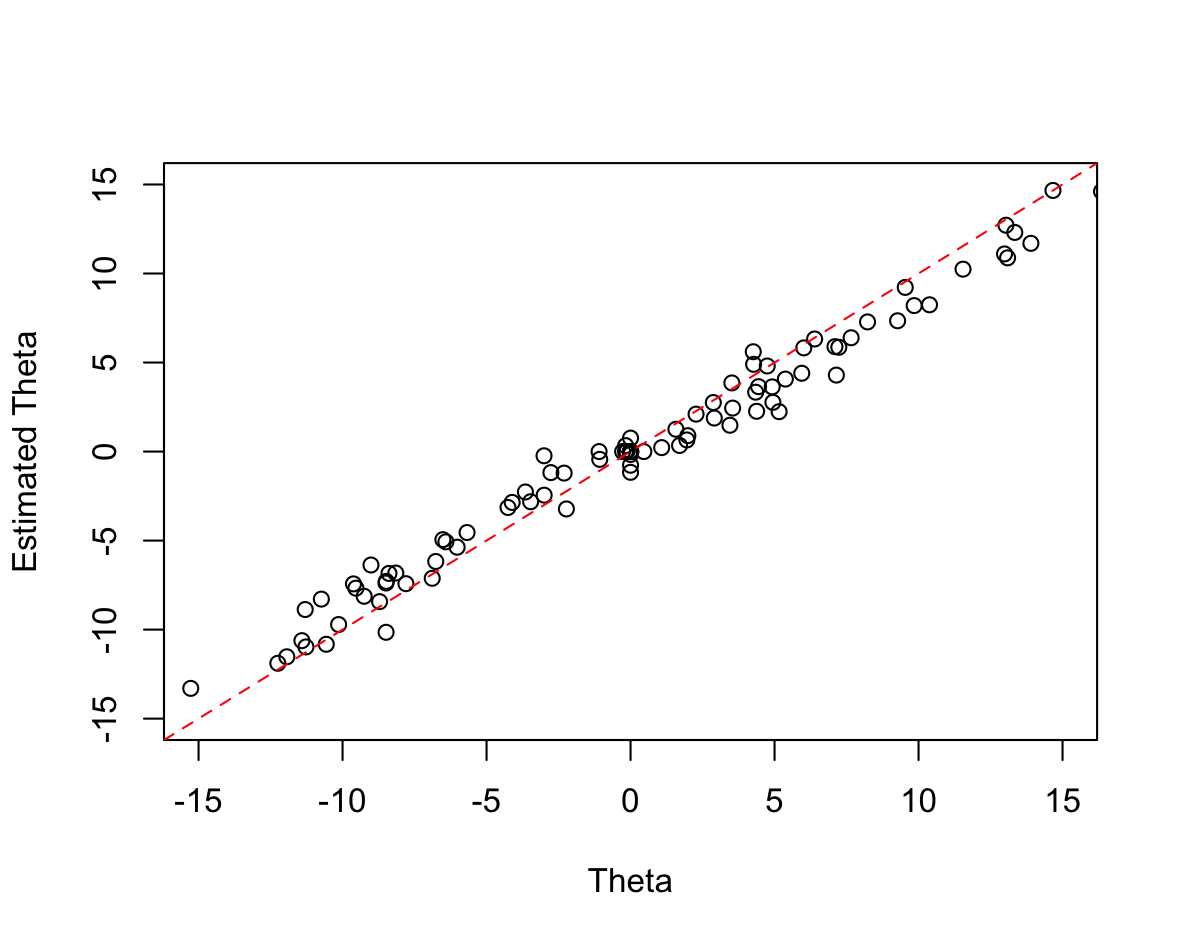
\includegraphics[width=\linewidth]{R_Code/Fig/P1B_K_09_l_1.png}
				\caption{$\lambda=1$ and $K=0.9$}
			\end{subfigure}
			\begin{subfigure}[h]{0.3\linewidth}
			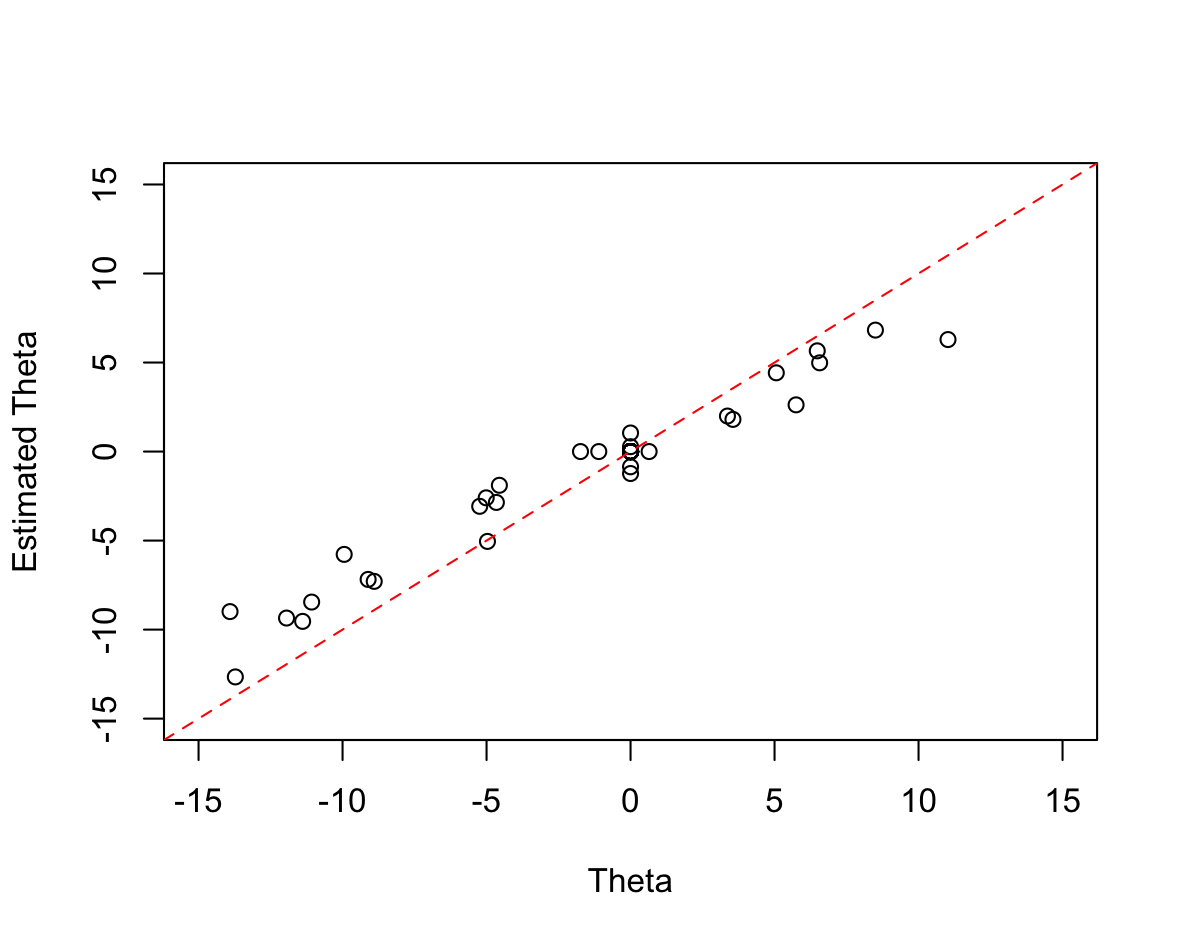
\includegraphics[width=\linewidth]{R_Code/Fig/P1B_K_03_l_2.png}
			\caption{$\lambda=2$ and $K=0.3$}
		\end{subfigure}
		\begin{subfigure}[h]{0.3\linewidth}
			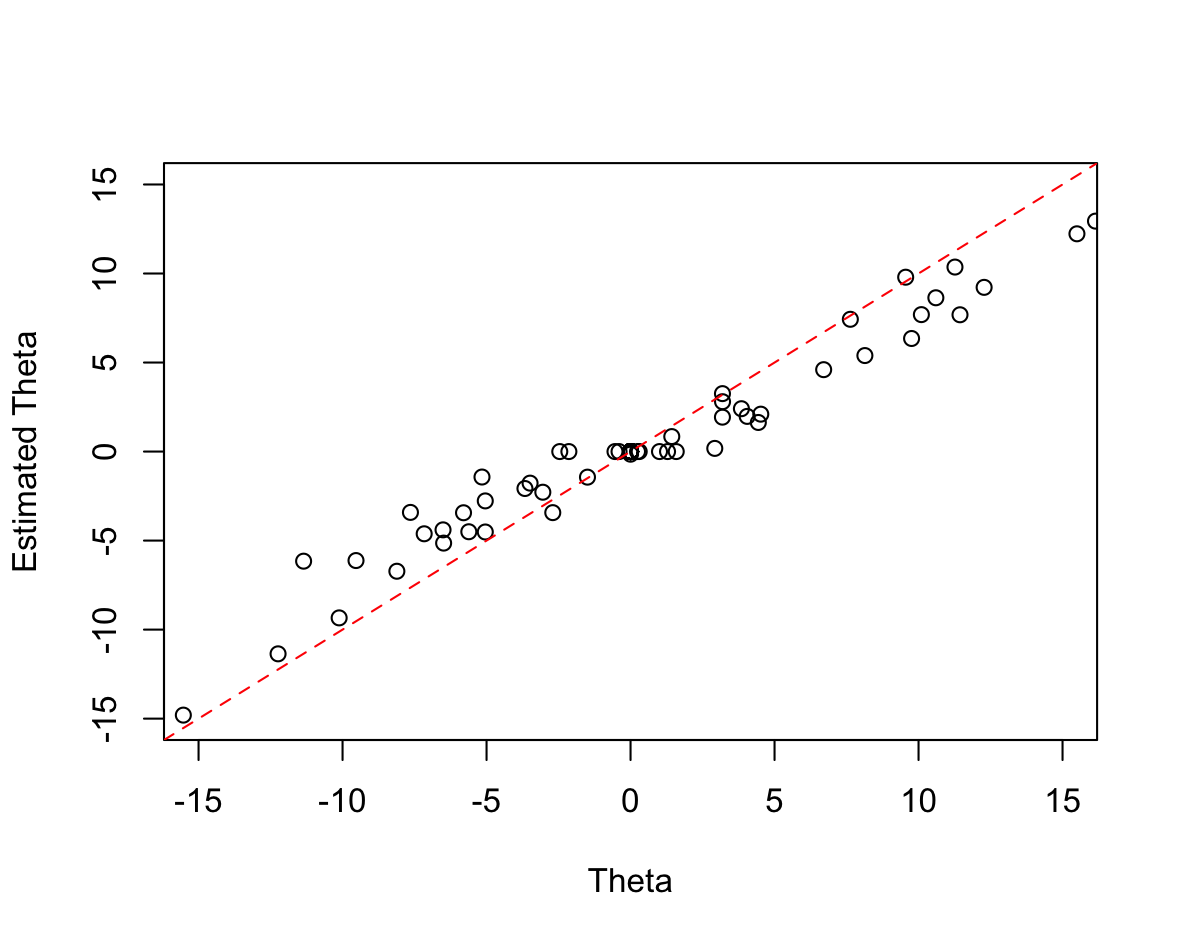
\includegraphics[width=\linewidth]{R_Code/Fig/P1B_K_05_l_2.png}
			\caption{$\lambda=2$ and $K=0.5$}
		\end{subfigure}
		\begin{subfigure}[h]{0.3\linewidth}
			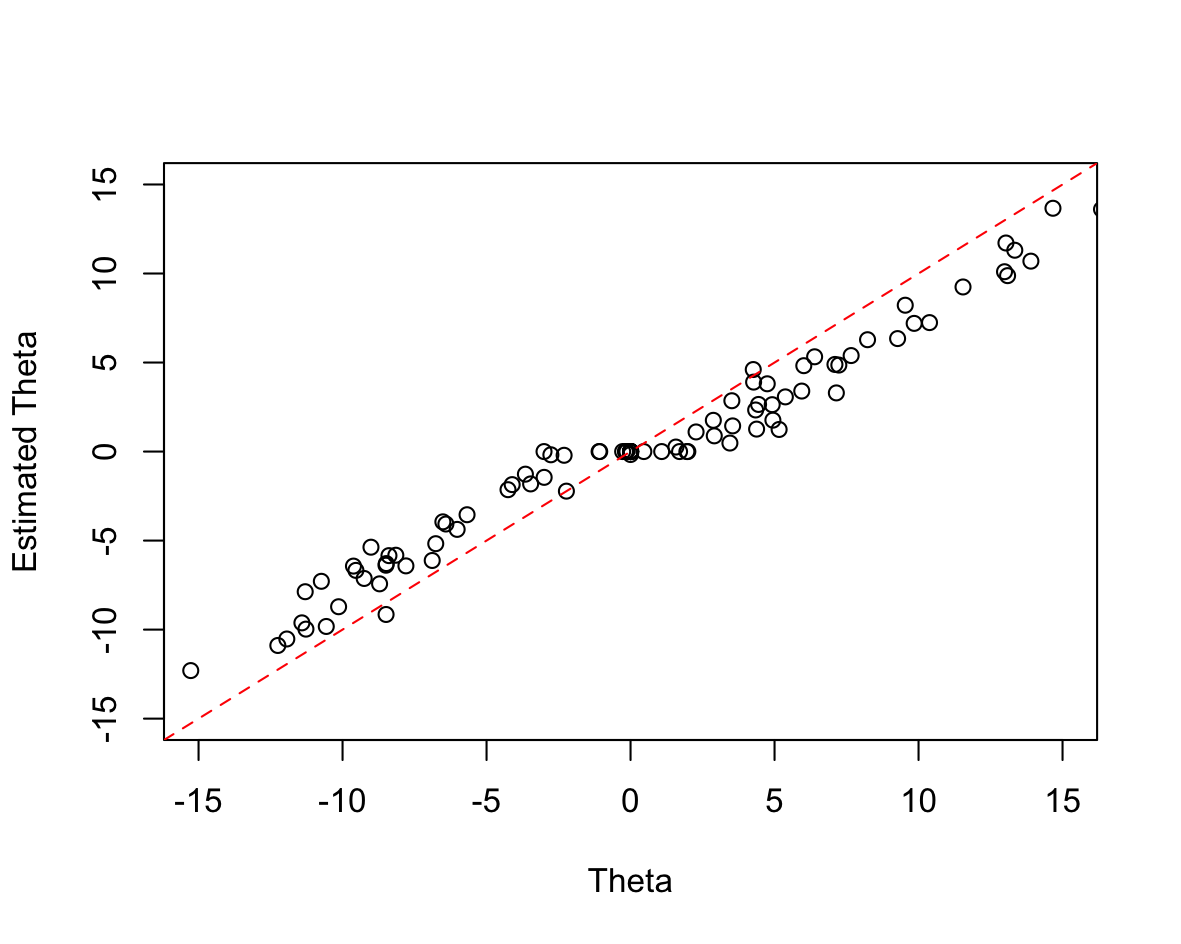
\includegraphics[width=\linewidth]{R_Code/Fig/P1B_K_09_l_2.png}
			\caption{$\lambda=2$ and $K=0.9$}
		\end{subfigure}
		\begin{subfigure}[h]{0.3\linewidth}
			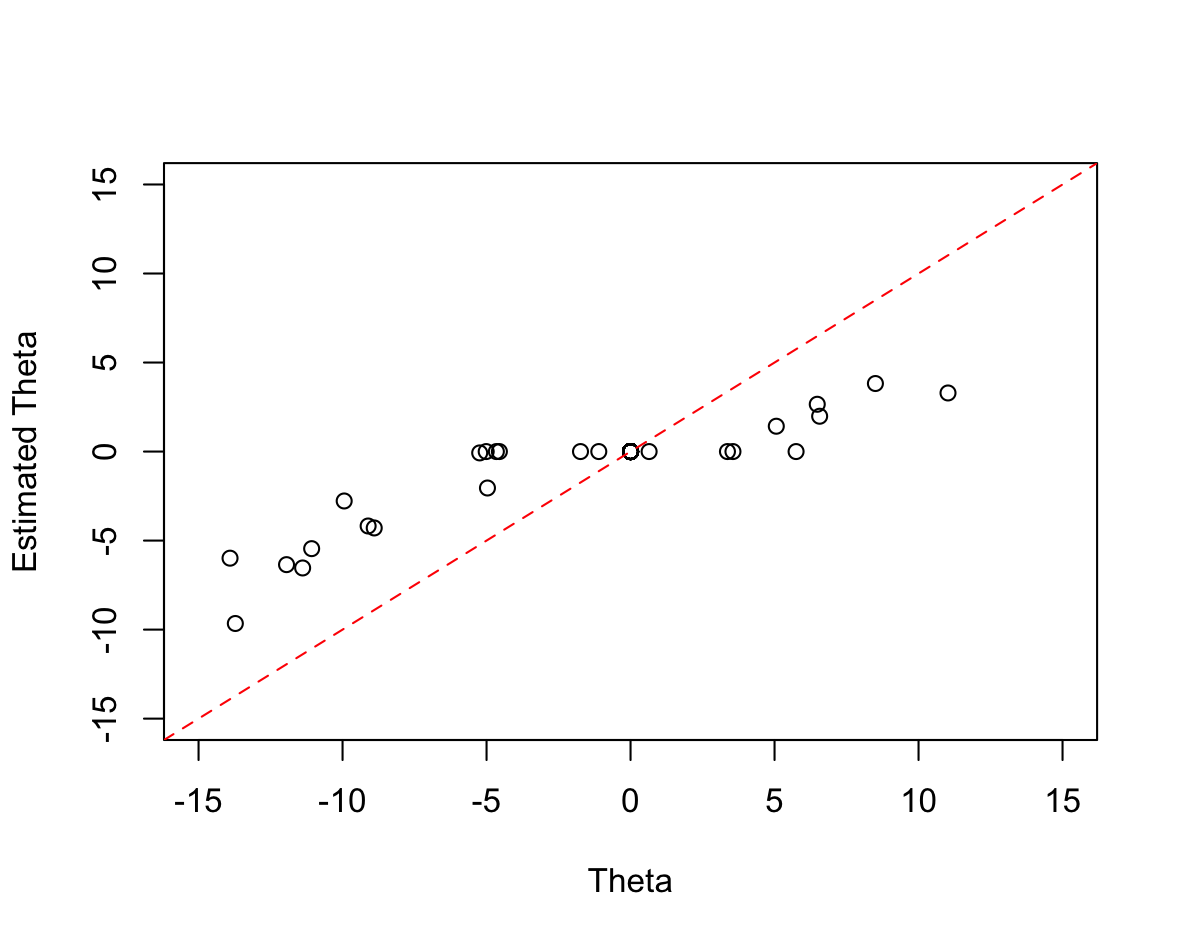
\includegraphics[width=\linewidth]{R_Code/Fig/P1B_K_03_l_5.png}
			\caption{$\lambda=5$ and $K=0.3$}
		\end{subfigure}
		\begin{subfigure}[h]{0.3\linewidth}
			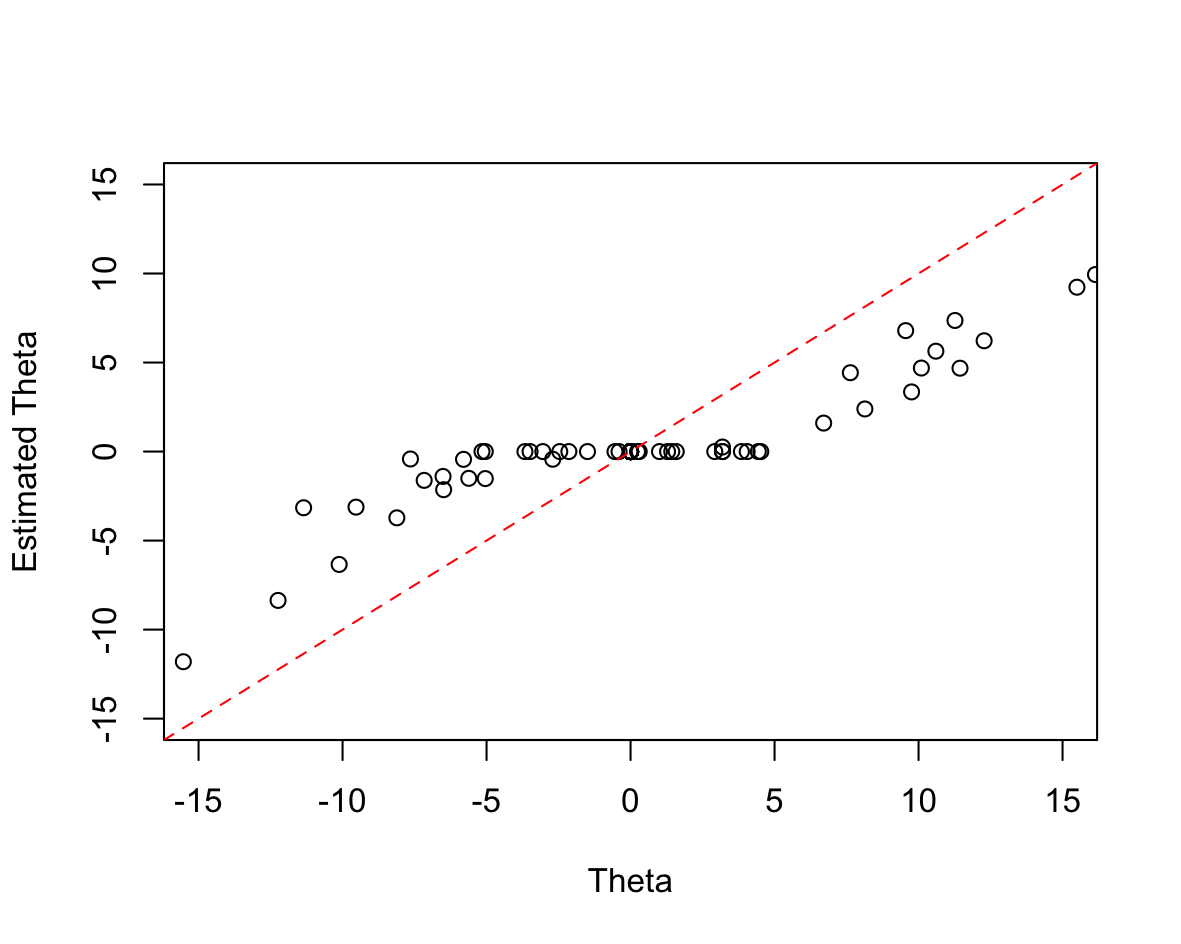
\includegraphics[width=\linewidth]{R_Code/Fig/P1B_K_05_l_5.png}
			\caption{$\lambda=5$ and $K=0.5$}
		\end{subfigure}
		\begin{subfigure}[h]{0.3\linewidth}
			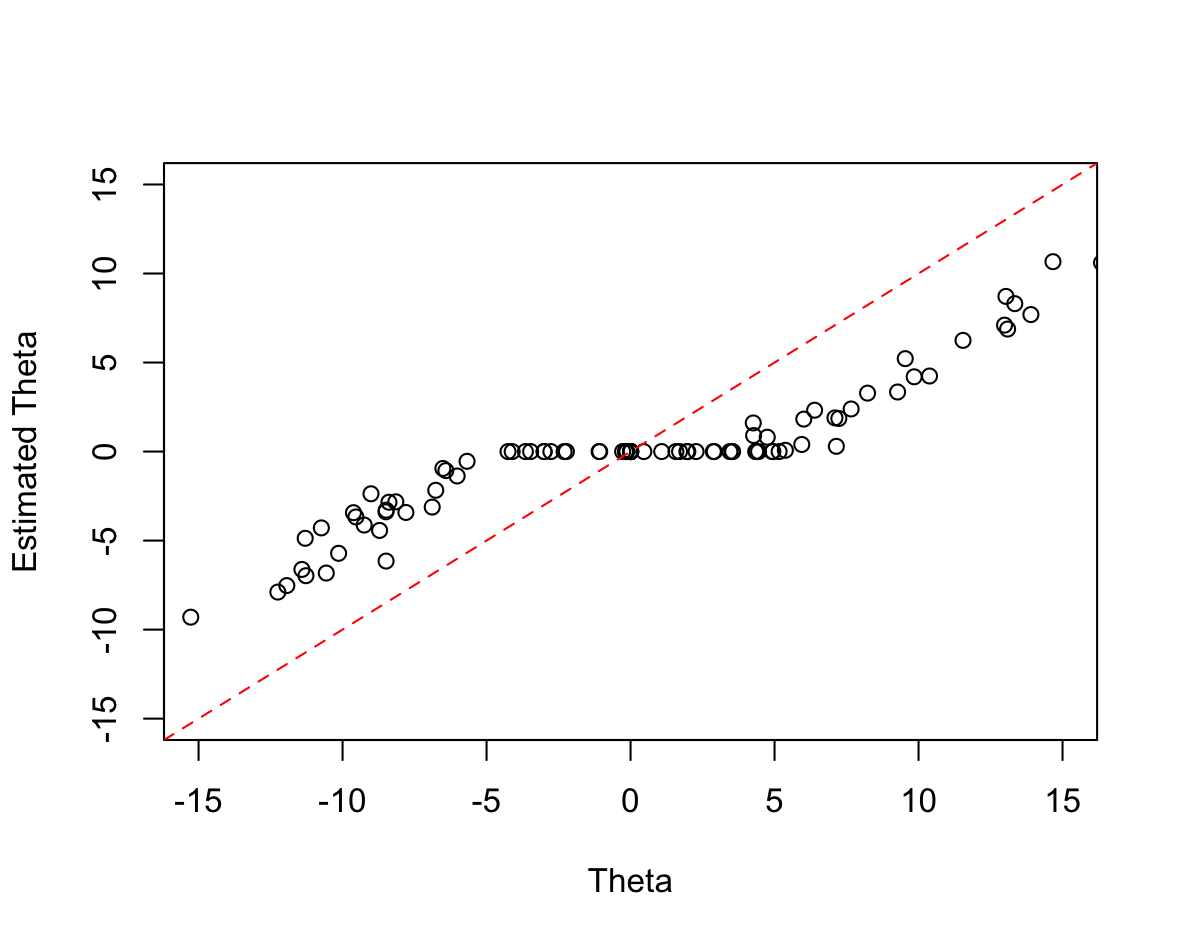
\includegraphics[width=\linewidth]{R_Code/Fig/P1B_K_09_l_5.png}
			\caption{$\lambda=5$ and $K=0.9$}
		\end{subfigure}
			\caption{ $\widehat{\theta}$  and $\theta_i$ with different  $\lambda$ and sparsity ($K$) values}
			\label{fig:Fig1}
		\end{center}
	\end{figure}
	\newpage
	\item Plot the mean-squared error of your estimate as a function of $\lambda$:
	$$
	\mbox{MSE}(\lambda) = \frac{1}{n} \sum_{i=1}^n  \left\{ \widehat{\theta}(y_i) - \theta_i \right\}^2 \, .
	$$
	Make sure that the MSE actually obtains a minimum across the grid of $\lambda$ values you have chosen.
	Try this for several different configurations of $\theta$.  

Note: like I said, this is an intuition-building exercise.  You could never choose $\lambda$ this way for a real problem, because it requires knowledge of the truth.\\

\lstinputlisting[language = R, firstline=61, lastline=80]{R_Code/Part_1B.R}
\newpage
How does the optimal $\lambda$ change as the sparsity in $\theta$ changes?\footnote{Here it's enough to assess the optimal $\lambda$ using the good old-fashioned ``plot and point'' strategy for optimization.  That is, you plot the function, point at the minimum, and say proudly, ``Here's the minimum.''}

We can observe from Figure 4 that as we decrease the sparsity (greater $K$), we obtain lower $\lambda$ values. This means that there is not need to force sparsity.\\


		\begin{figure}[H]
		\begin{center}
			\begin{subfigure}[h]{0.4\linewidth}
				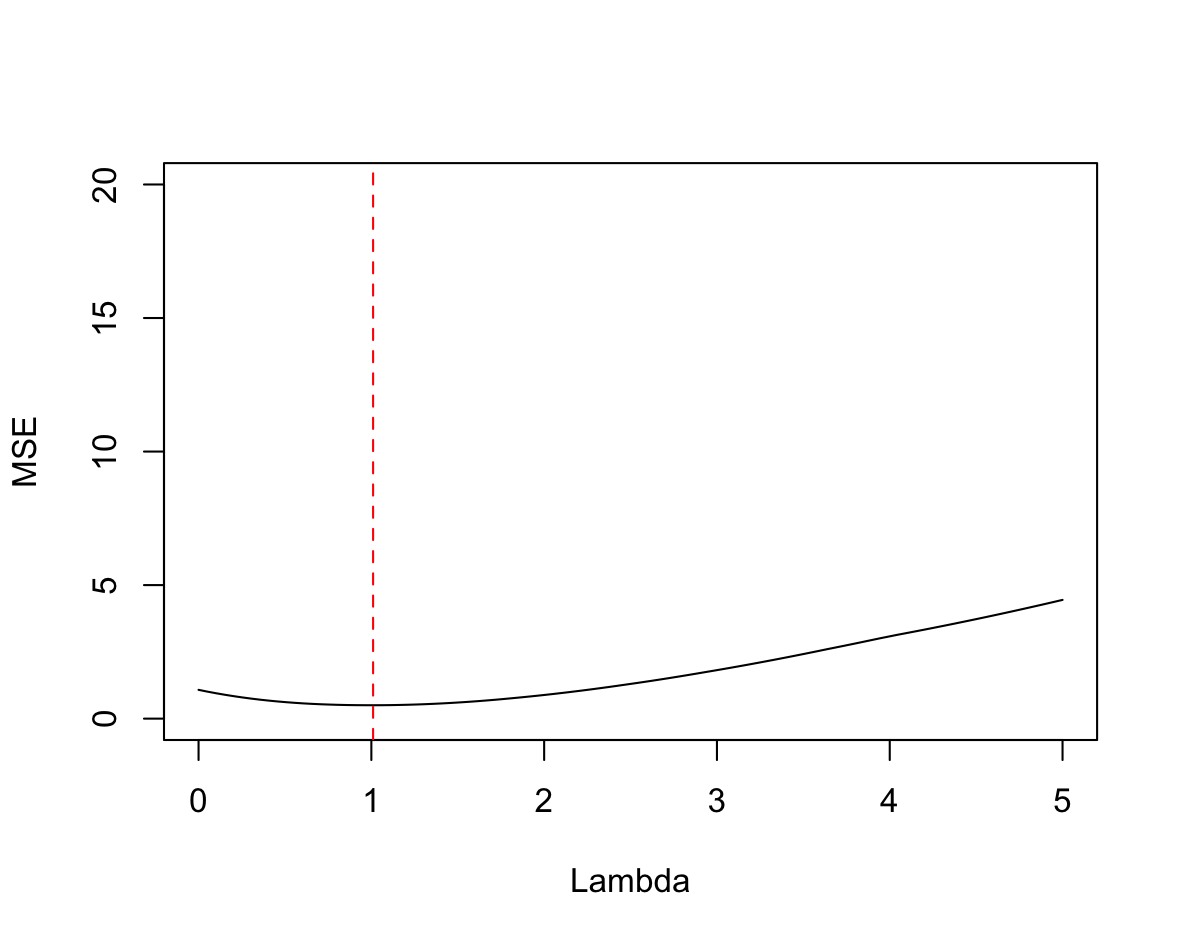
\includegraphics[width=\linewidth]{R_Code/Fig/P1BB_K_03.png}
				\caption{$K=0.3$, and Minimum $\lambda = 1.0101$}
			\end{subfigure}\\
			\begin{subfigure}[h]{0.4\linewidth}
				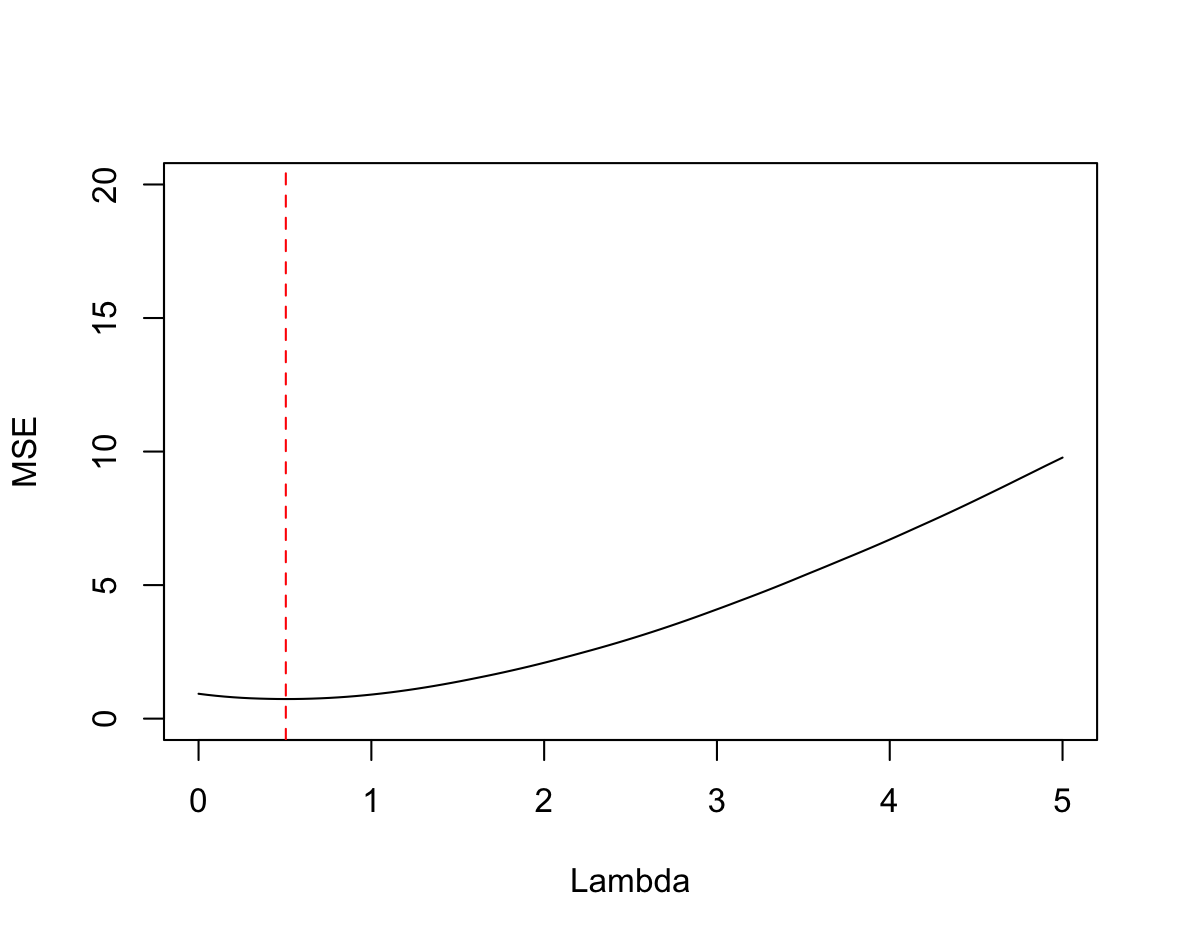
\includegraphics[width=\linewidth]{R_Code/Fig/P1BB_K_05.png}
				\caption{$K=0.5$, and Minimum $\lambda = 0.5050$}
			\end{subfigure}\\
			\begin{subfigure}[h]{0.4\linewidth}
				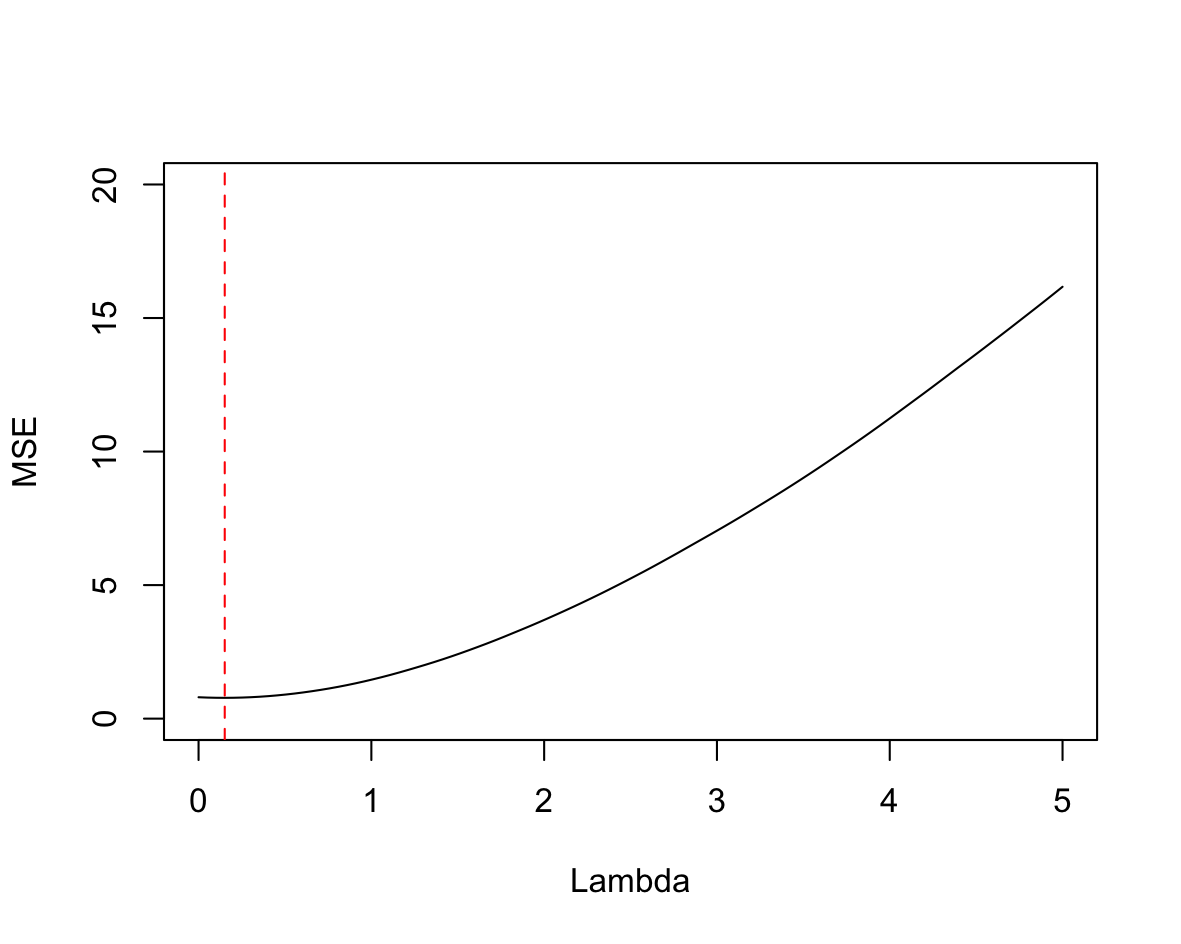
\includegraphics[width=\linewidth]{R_Code/Fig/P1BB_K_09.png}
				\caption{$K=0.9$, and Minimum $\lambda = 0.1515$}
			\end{subfigure}
		\caption{ Mean-squared error (MSE)  for different $\lambda$ and sparsity ($K$) values}
		\label{fig:Fig1}
		\end{center}
		\end{figure}

\end{enumerate}
\end{enumerate}

\newpage
\section{The lasso}

Although  a soft-thresholding approach to the normal-means problem is actually very useful in practice, this utility is not immediately apparent.  On the other hand, a generalization of this idea to regression, called the lasso,\footnote{``Lasso'' stands for ``least absolute shrinkage and selection operator.  It was proposed in a \url{http://statweb.stanford.edu/~tibs/lasso/lasso.pdf}{classic paper} by Robert Tibshirani.} both looks and is immediately useful.

Consider the standard linear regression model
$$
y = X \beta + e \, ,
$$
where $y$ is an $n$-vector of responses, $X$ is an $n \times p$ features matrix whose $i$th row $x_i$ is the vector of features for observation $i$, and $e$ is a vector of errors/residuals.

The lasso involves estimating $\beta$ as the solution to the penalized least-squares problem\footnote{Note: some will write the ``fit'' part of the objective function as
$$
\frac{1}{2n} \Vert y - X \beta \Vert_2^2 \, ,
$$
where $n$ is the sample size.  Translating between these two problems involves multiplying $\lambda$ by a factor of $n$.
}
$$
\hat{\beta} = \arg \min_{\beta} \; \frac{1}{2} \Vert y - X \beta \Vert_2^2 + \lambda \Vert \beta \Vert_1 \, ,
$$
where $\Vert \beta \Vert_1$ is the $\ell_1$ (pronounced ``ell one'') norm of the coefficient vector:
$$
\Vert \beta \Vert_1 = \sum_{j=1}^p |\beta_j| \, .
$$
As you can see, the penalty function is just like the absolute-value penalty you used on the normal-means problem, generalized to the vector case.  And just as in in the normal means problem, this penalty function will have the effect of both selecting a set of nonzero $\beta_i$'s (i.e.~sparsifying the estimate) as well as shrinking the nonzero $\beta_i$'s toward 0.  The bigger $\lambda$, the more aggressive the shrinkage effect.

Note: we typically leave the intercept in a lasso fit unpenalized.  We can accomplish this by explicitly introducing an intercept, e.g. writing the objective as
$$
\frac{1}{2n} \Vert y - (\alpha \mathbf{1} + X \beta) \Vert_2^2 + \lambda \Vert \beta \Vert_1 \, ,
$$
where $\alpha$ is a scalar intercept and $\mathbf{1}$ is a vector of all 1's.  Or we can leave the problem in its original form above, and assume that both the response variable $y$ and all columns of the predictor matrix have been standardized have a mean of 0 (in which case there is no need for an explicit intercept).  For the rest of these exercises, we'll assume that the variables have been standardized in this way.

To read more about lasso regression, consult Chapter 3.4.2 of \textit{The Elements of Statistical Learning}, or the original paper \footnote{\url{http://statweb.stanford.edu/~tibs/lasso/lasso.pdf}} by Robert Tibshirani.

\newpage

\begin{enumerate}[label=(\Alph*)]

\item For now, we won't worry about \textit{how} the lasso model is fit.  Instead, we'll use pre-existing software to fit it:
\begin{description}
	\item[In R:] the package \verb|glmnet|, described here \footnote{\url{https://web.stanford.edu/~hastie/glmnet/glmnet_alpha.html}}.
	\item[In Python:] \verb|sklearn.linear_model.Lasso| in scikit-learn \footnote{\url{http://scikit-learn.org/stable/index.html}}.
\end{description}
That way, we can build intuition for its properties, as well as come to an appreciation for some of the statistical questions that arise in fitting the model.  If you want to learn about how these functions fit the lasso model, read about coordinate descent in Chapter 3.8.6 of \textit{The Elements of Statistical Learning}, or in this paper \footnote{\url{http://arxiv.org/pdf/0708.1485.pdf}}.

Download the data on diabetes progression in 442 adults from the Data folder on the class website.  There are two files here.
\begin{description}
	\item[diabetesY.csv:] the response variable for each patient.  This is the result of a blood test that provides a quantitative measure of disease progression one year after baseline (e.g.~at diagnosis).
	\item[diabetesX.csv:] 10 baseline patient variables, age, sex, BMI, cholestorol measurements, etc.  Also here are all 10 quadratic terms of the form $x_{ij}^2$ and all 45 possible pairwise interactions of the form $x_{ij} \cdot x_{ik}$.  This leads to 65 total variables: 10 linear main effects and 10 quadratic main effects from the baseline variables, and 45 interactions (45 = 10 choose 2).  The 10  baseline variables are standardized to have zero mean and unit Euclidean norm (i.e.~the sum of squared entries in the first 10 columns is 1).
\end{description}

Fit the lasso model across a range of $\lambda$ values (which \verb|glmnet| does automatically) and plot the solution path $\hat{\beta}_{\lambda}$ as a function of $\lambda$, just like Figure 3.10 in \textit{Elements}.\footnote{For Python users, there is a ``warm start'' option to the lasso fitter, which can use the last solution as an initial guess for the next call.  This is great for fitting a solution path.}  (Note: your horizontal axis can just be $\lambda$, or $\log \lambda$.)

In addition, you should track the in-sample mean-squared prediction error of the fit across the solution path:
$$
\mathrm{MSE}(\hat \beta_{\lambda}) = \frac{1}{n} \sum_{i=1}^n (y_i - x_i^T \hat \beta_{\lambda}^2) = \frac{1}{n} \Vert y - X \hat \beta_{\lambda} \Vert_2^2 \, .
$$

\newpage
\textbf{Solution}

The solution is presented in the file $Part\_2.R$,
\lstinputlisting[language = R, firstline=6, lastline=30]{R_Code/Part_2.R}

\begin{figure}[H]
\begin{center}
	\begin{subfigure}[h]{0.7\linewidth}
		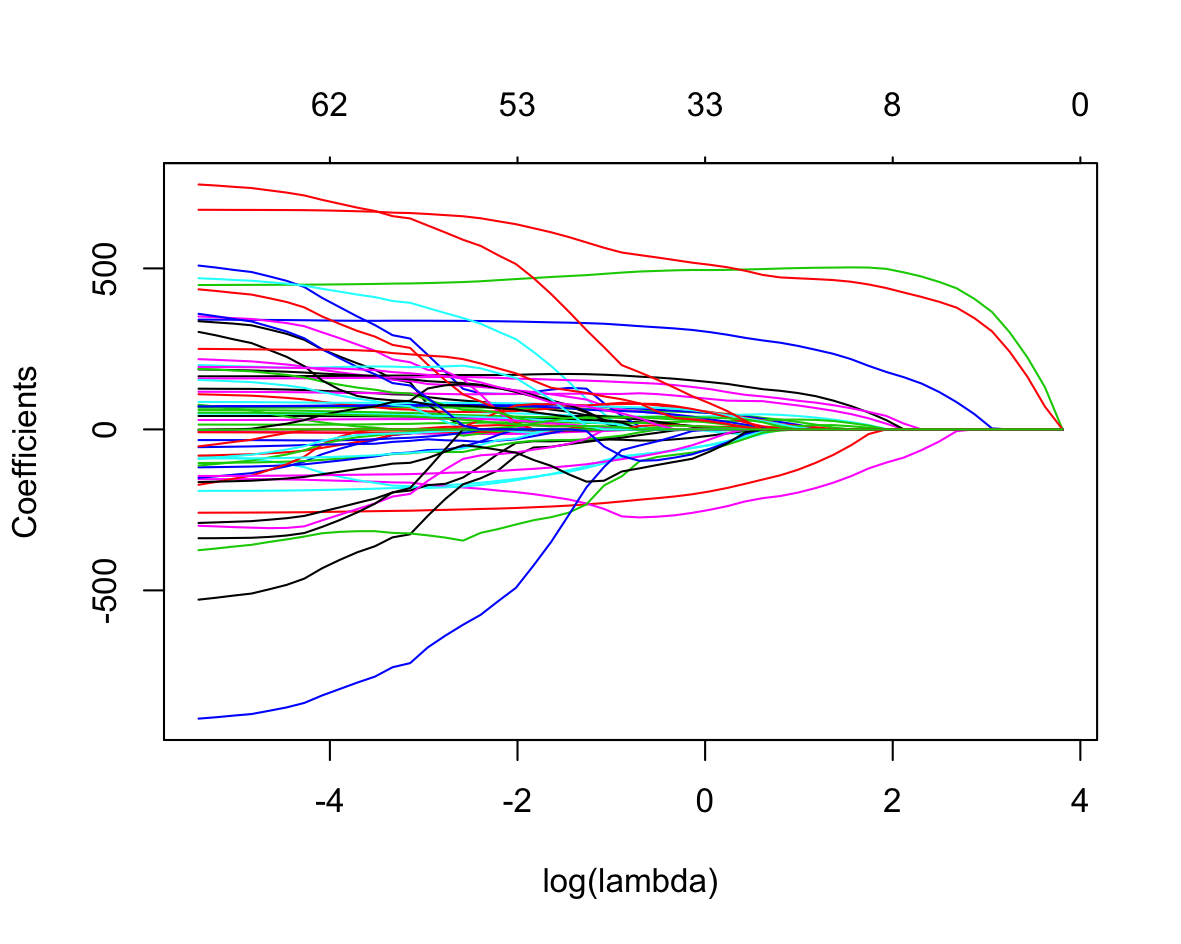
\includegraphics[width=\linewidth]{R_Code/Fig/P2A_Lasso.png}
		\caption{Profiles of lasso coefficients}
	\end{subfigure}\\
	\begin{subfigure}[h]{0.7\linewidth}
		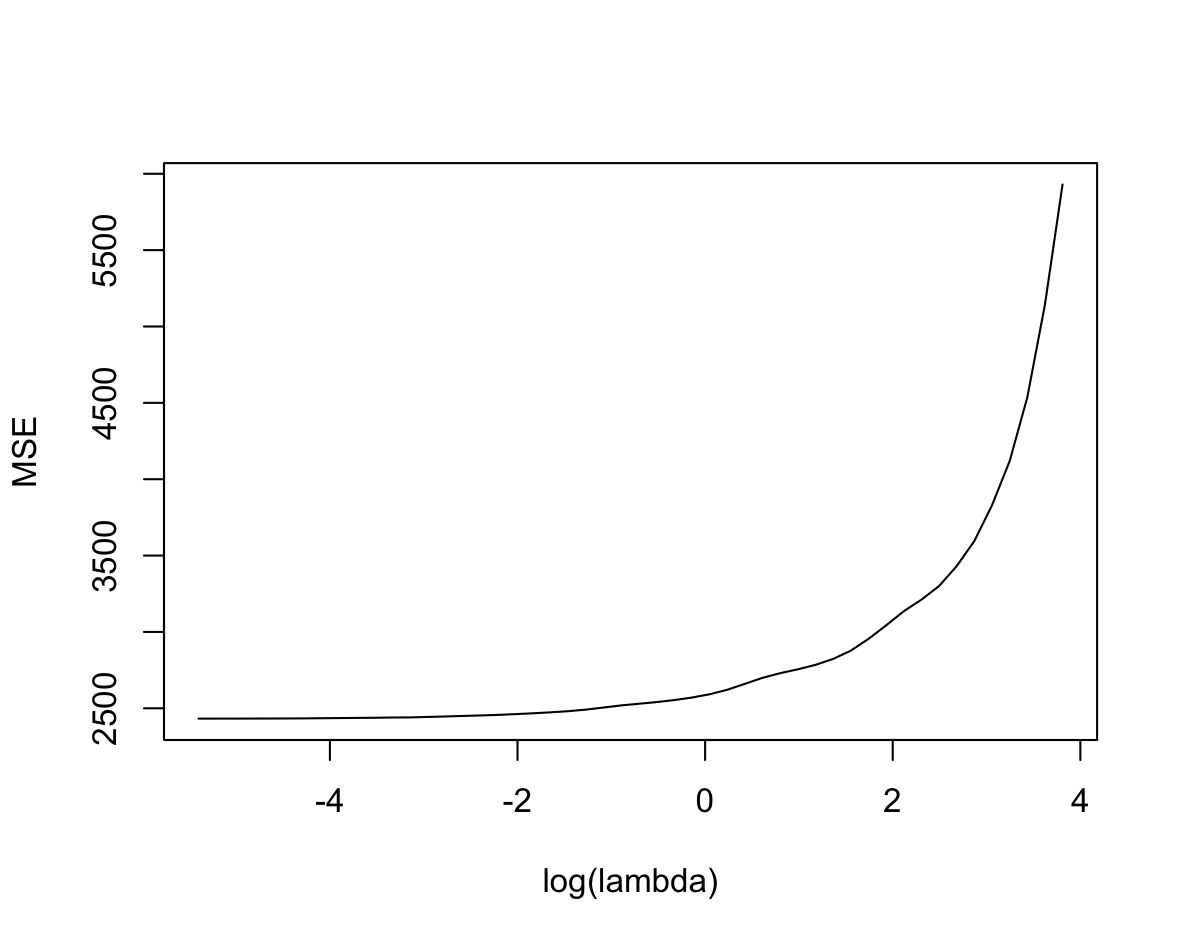
\includegraphics[width=\linewidth]{R_Code/Fig/P2A_MSE.png}
		\caption{In-sample mean-squared prediction error of the fit }
	\end{subfigure}\\
	\caption{ Lasso Regression}
	\label{fig:Fig1}
\end{center}
\end{figure}



\newpage
\item A natural way to choose $\lambda$ is to minimize the expected out-of-sample prediction error.  Suppose that $(x_{\star}, y_{\star})$ is a future data point from the same population/data-generating process as the original data.  The goal would be to make the expected error
$$
\mathrm{MOOSE}(\hat{\beta}_{\lambda}) =  E \left\{ (y_{\star} - \hat{y}_{\star} )^2 \right\} = E \left\{ (y_{\star} - x_\star^T \hat{\beta}_{\lambda} )^2 \right\} 
$$
as small as possible.  Here the expected value is taken under what probability distribution generates $(x,y)$ pairs, and ``MOOSE'' stands for mean out-of-sample squared error.\footnote{MOOSE is not a standard acronym, but shouldn't it be?!}  Of course, we don't have any ``future data'' lying around, so we have to estimate this quantity using the data we have.  The in-sample mean-squared error, $\mathrm{MSE}(\hat \beta_{\lambda})$, is generally an optimistic estimate of this quantity: out-of-sample error tends to be worse, on average, than in-sample error, and we need some way of quantifying how much worse.

One way is using cross validation.  If you're unfamiliar with this concept, read about it in Chapter 7.10 of \textit{Elements} (you may need to track back to the beginning of chapter 7 to pick up their notation).  The essential idea is to split your data set into ``training'' and ``testing'' sets.  Then you fit the model on the training set, and compute the average out-of-sample prediction error on the test set.  This provides an estimate of the MOOSE.  (You actually average this estimate over multiple such train/test splits, to reduce the influence of randomness in the split itself.)

I leave it to you to figure out the details of cross validation, including how big your training and testing sets should be.  Again, Chapter 7.10 \textit{Elements} has good guidelines here.  Note: I expect you to write your own code for doing the train/test splits and computing out-of-sample error, wrapped around the base function for fitting the lasso regression model.   If you're in R, you can use the \verb|cv.glmnet| function as a sanity check on, but not a replacement for, your results.


\newpage
\textbf{Solution}

The solution is presented in the file $Part\_2.R$,
\lstinputlisting[language = R, firstline=32, lastline=83]{R_Code/Part_2.R}

Plot your cross-validated estimate of $\mathrm{MOOSE}(\hat{\beta}_{\lambda})$ across the solution path, as a function of $\lambda$.  How does it compare with the \textit{in-sample} mean-squared error from (A)?

We can observe the behavior similar to Figure 7.1 of the textbook (page 220). The in-sample MSE decreases as $\lambda$ decreases (over-fitting?), while the MOOSE presents a MSE minimum near $log(\lambda)=1.367$ or $\lambda=3.9222$.

\begin{figure}[H]
	\begin{center}
		\begin{subfigure}[h]{0.6\linewidth}
			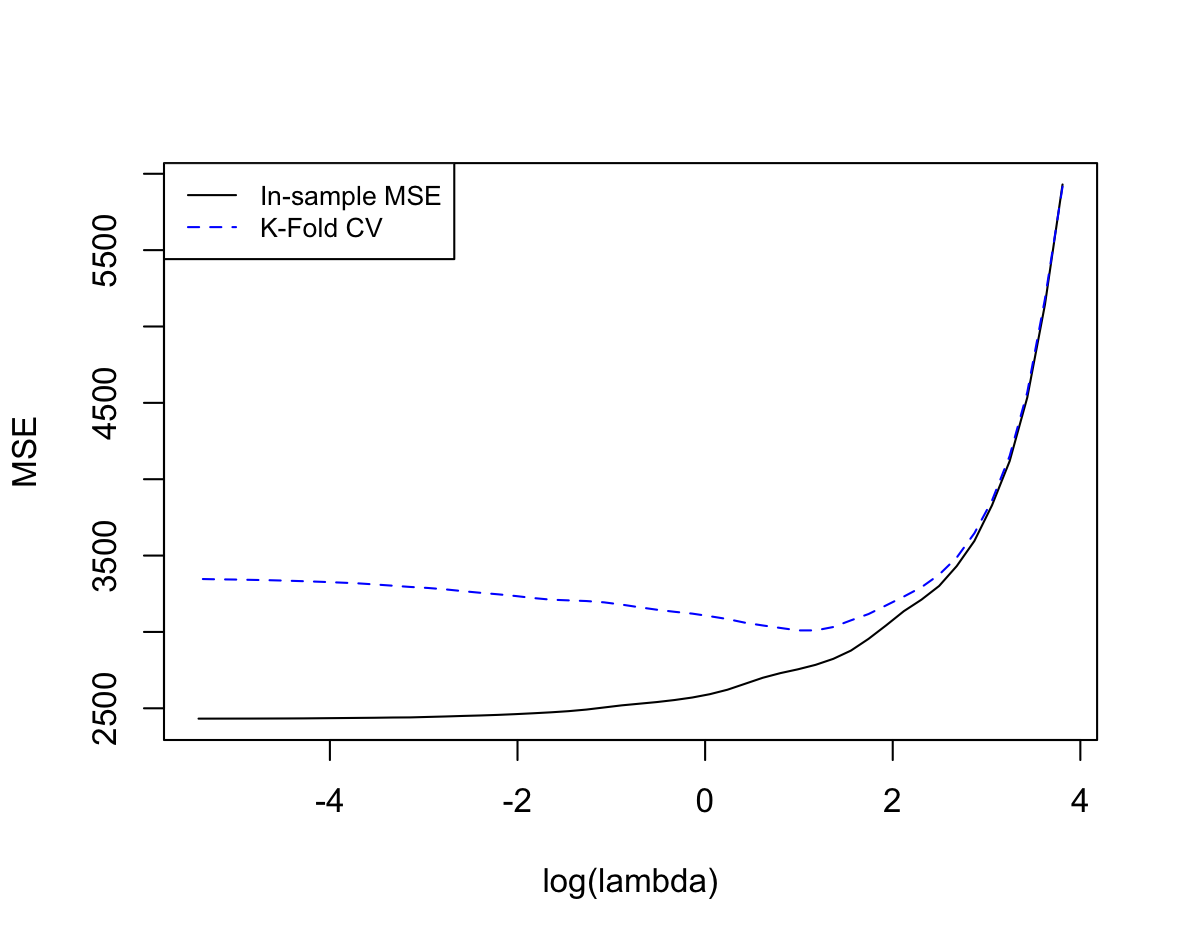
\includegraphics[width=\linewidth]{R_Code/Fig/P2A_MSE2.png}
			\caption{K-Fold Cross-Validation MOOSE compared to in-sample MSE}
		\end{subfigure}\\
		\begin{subfigure}[h]{0.6\linewidth}
			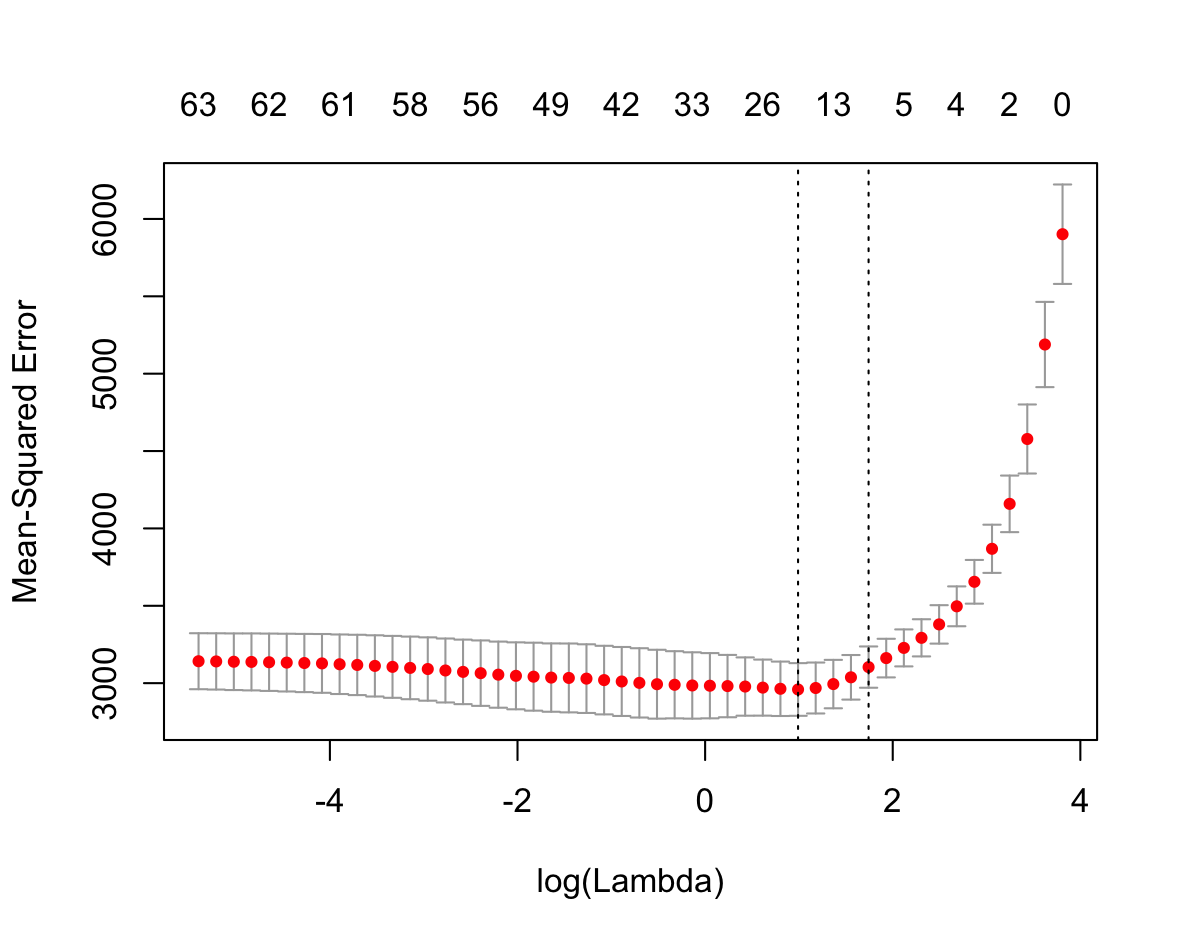
\includegraphics[width=\linewidth]{R_Code/Fig/P2A_MSE3.png}
			\caption{K-fold cross-validation MOOSE obtained using CV.glmnet (sanity check)}
		\end{subfigure}\\
		\caption{Cross validation}
		\label{fig:Fig1}
	\end{center}
\end{figure}


\newpage
\item Cross validation is one particularly simple way, based on the idea of resampling your data, to estimate the generalization error of a model.  (Its reliance on resampling means that it shares a lot in common with the bootstrap \footnote{\url{https://en.wikipedia.org/wiki/Bootstrapping_(statistics)}} as a way to estimate the standard error of a model parameter.)

However, cross-validation isn't the only way to estimate generalization error.  Another such way is called the $C_p$ statistic, proposed by Collin Mallows (and therefore often called \textit{Mallows' $C_p$}).  For a linear regression model, the $C_p$ statistic is defined as
$$
C_p(\hat{\beta}_\lambda) = \mathrm{MSE}(\hat \beta_{\lambda}) + 2 \cdot \frac{s_{\lambda}}{n} \hat \sigma^2 \, ,
$$
where $s_{\lambda}$ is the degrees of freedom of the fit (i.e.~the number of nonzero parameters selected at that particular value of $\lambda$), and $\hat \sigma^2 = \mathrm{var}(\epsilon)$ is an estimate of the residual variance.  You can interpret the $C_p$ statistic as the in-sample mean-squared error, plus a penalty for in-sample optimism.  As you add parameters to a regression model, MSE goes down and the penalty goes up. 


\paragraph{Note 1:} In general, the main tradeoffs between cross-validation and the $C_p$ statistic are these:
\begin{itemize}
	\item  Cross validation is more robust, in the sense that it does not require that you believe the model is right in order to provide a decent estimate of generalization error.  But it is more computationally expensive, and less statistically efficient if the underlying model is approximately right.
	\item $C_p$ (or related statistics like AIC, BIC, etc) has the advantage that it does not require the repeated ``split and refit'' of cross validation, and is thus less computationally expensive.  It is also more statistically efficient if the model is right.  But it is not as robust as cross validation to violations of the underlying modeling assumptions (like linearity).
\end{itemize}
See the ``Estimating prediction error'' paper below for more detail.

\paragraph{Note 2:} You need to plug an estimate of $\sigma^2$ into the $C_p$ statistic.  A typical way to proceed is to use the unbiased estimate of $\sigma^2$ arising from the ordinary-least-squares solution $\hat \beta_{\mathrm{OLS}}$:
$$
\hat{\sigma}^2 = \frac{1}{n - p} \sum_{i=1}^n (y_i - x_i^T \hat \beta_{\mathrm{OLS}}^2) \, ,
$$
i.e.~the model fit to all $p$ variables.  Note: this assumes no intercept due to variable centering; if you have an intercept, substract an extra degree of freedom in the denominator (i.e.~$n-p-1$).

Another natural estimator for the residual variance $\sigma^2$ is to use, for each $\lambda$, the formula
$$
\hat{\sigma}^2_{\lambda} = \frac{1}{n - s_{\lambda}} \sum_{i=1}^n (y_i - x_i^T \hat \beta_{\lambda}^2) \, ,
$$
where again $s_{\lambda}$ is the degrees of freedom of the fit.  This formula parallels the usual formula given for an unbiased estimate of the error variance for the OLS model.

To be honest, I am not sure if there is any theory supporting the use of one or the other of these variance estimators in the context of the $C_p$ statistic.  Mostly I have seen people use the former estimator, based on the OLS fit.  The relevant papers here are these, also linked from the class website:
\begin{itemize}
	\item Degrees of freedom of the lasso fit \footnote{\url{https://projecteuclid.org/euclid.aos/1194461726)}}.
	\item Estimating the residual variance from the lasso fit \footnote{\url{https://arxiv.org/abs/1311.5274}}.
	\item Estimating prediction error \footnote{ \url{https://people.eecs.berkeley.edu/~jordan/sail/readings/archive/efron_Cp.pdf}}.  This paper has a much more extensive discussion and list of references about the idea of the $C_p$ statistic and its generalizations.
\end{itemize}

\vspace{10mm}
\textbf{Solution}

The solution is presented in the file $Part\_2.R$,
\lstinputlisting[language = R, firstline=85, lastline=122]{R_Code/Part_2.R}


Compute (and plot) the $C_p$ statistic across the solution path, as a function of $\lambda$.  How does it compare to the in-sample MSE, and to the cross-validated estimate of generalization error from (B)?  Show these all on the same plot.  Do they lead to similar choices of $\lambda$?

\vspace{2mm}
Figure 7 shows the results for Mallow's Cp compared to K-fold cross-validation MOOSE and in-sample MSE. We can observe that Mallow's Cp follows the K-fold method and presents similar minimum value of $\lambda$ but it's less computationally expensive.

\begin{figure}[H]
	\begin{center}
		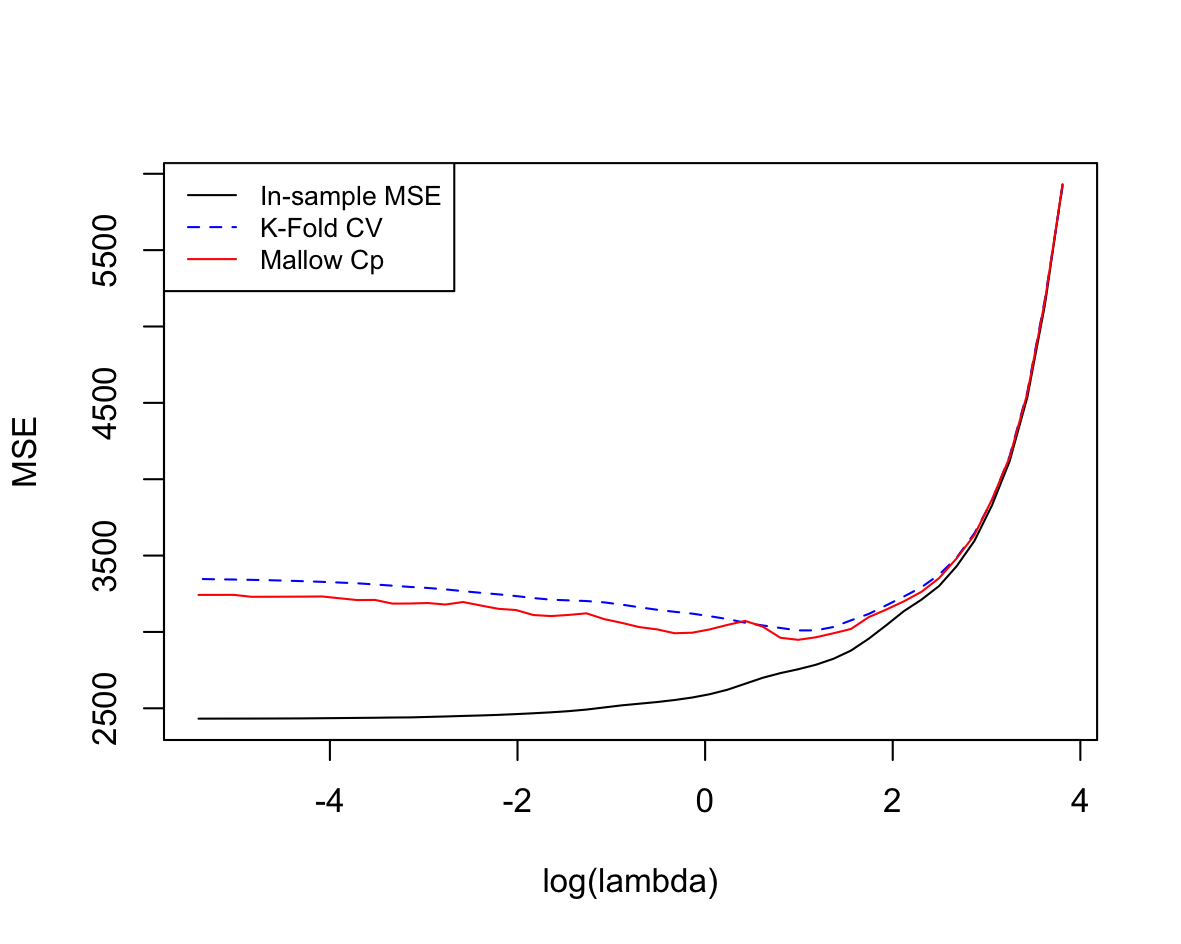
\includegraphics[width=0.8\linewidth]{R_Code/Fig/P2A_MSE4.png}
		\caption{Mallow's $C_p$ statistic compared to K-fold cross-validation MOOSE and in-sample MSE}
	\end{center}
\end{figure}

\end{enumerate}
\end{document}